\documentclass[a4paper,10t]{article}
\usepackage[utf8]{inputenc}
\usepackage{indentfirst}
\usepackage{times}
\usepackage[T1]{fontenc}
\usepackage[affil-it]{authblk}
\usepackage{authblk}
\usepackage{amssymb,amsmath,amsthm,ragged2e}
\usepackage{setspace,lipsum}
\usepackage[pdftex]{color,graphicx}
\usepackage{adjustbox}
\usepackage{lmodern,caption}
\usepackage{booktabs,array}
\usepackage{epstopdf}
\usepackage[figuresright]{rotating}
\usepackage{pgfplots} 
\usepackage{pgfgantt}
\usepackage{pdflscape}
\usepackage{algpseudocode}
\pgfplotsset{compat=newest} 
\pgfplotsset{plot coordinates/math parser=false}
\DeclareGraphicsRule{.tif}{png}{.png}{`convert #1 `dirname #1`/`basename #1 .tif`.png}
\usepackage{array,longtable}
\usepackage[top=3cm, bottom=2cm, left=2cm, right=2cm]{geometry}
\newcommand{\otoprule}{\midrule[\heavyrulewidth]}
\newcolumntype{Z}{>{\centering\arraybackslash}X}
\usepackage{latexsym,hhline}
\usepackage[round]{natbib} % use author-year citation style
\usepackage[colorlinks=true,allcolors=blue]{hyperref} % simplify color scheme ...
%\usepackage{cite}
\usepackage{setspace}
\onehalfspacing
\DeclareMathOperator{\diag}{diag}
\DeclareMathOperator{\Ima}{Im}
\DeclareCaptionLabelSeparator{horse}{:\quad} % change according to your needs
\captionsetup{
	labelsep = horse,
	figureposition = bottom % proper spacing between figure and caption
}
\usepackage{tikz,color,listings,float,booktabs,enumerate,multirow,multicol,subcaption}
\usepackage{parskip}
\setlength{\parindent}{15pt}
\usepackage{bigstrut,hyperref,tabularx,ctable,array,longtable,tikz}
\hypersetup{
	pdftitle={TITLE},
	pdfauthor={AUTHOR},
	pdfsubject={SUBJECT},
	pdfkeywords={KEYWORD} {KEYWORD} {KEYWORD},
	colorlinks=true,
	linkcolor=blue,
	citecolor=blue,
	filecolor=magenta,
	urlcolor=blue
}
\newtheorem{theorem}{Theorem}
\newtheorem{proposition}{Proposition}
\newtheorem{lemma}{Lemma}
\newtheorem{definition}{Definition}
\newtheorem{corollary}{Corollary}[theorem]
\usepackage{rotating}

% Real Number
\newcommand{\R}{\mathbb R}
% natural numbers
\newcommand{\Nat}{\mathbb N}
% complex numbers
\newcommand{\C}{\mathbb C}
\newcommand{\Pstar}{\mathbb{P}^{\ast}}
\newcommand{\E}{\mathbb{E}}
\newcommand{\Var}{\mathrm{Var}}
\newcommand{\Cov}{\mathrm{Cov}}
\newcommand{\Expect}{{\rm I\kern-.3em E}}
\usepackage[listings]{tcolorbox}
\tcbuselibrary{listings,theorems}
\usepackage{fancyheadings,xspace,amsmath,tikz-qtree}
\usetikzlibrary{matrix}

\usepackage[labelfont=bf]{caption} %% for the figure and Tables Caption%%
%\usepackage[textfont=bf]{caption}
\usepackage{threeparttable}
\usepackage{standalone}

\pgfplotsset{every axis/.append style={
%		axis x line=middle,    % put the x axis in the middle
%		axis y line=middle,    % put the y axis in the middle
%		axis line style={<->}, % arrows on the axis
%		xlabel={$x$},          % default put x on x-axis
%		ylabel={$y$},          % default put y on y-axis
		label style={font=\LARGE},
		ticklabel style={font=\LARGE}  
}}

\begin{document}

	
	\title{A Computationally Efficient Pairs Trading Strategy with Reinforcement Learning \\ or \\ A New Pairs Trading Strategy based on Reinforcement Lerarning}
	\author[]{ Fernando A. B. Sabino da Silva\thanks{\texttt{Department of Statistics, Federal University of Rio Grande do Sul, Porto Alegre, RS 91509-900, Brazil, e-mail: dasilvafbs@gmail.com}; Corresponding author.}}
	\author[]{Elton F. Sbruzzi\thanks{\texttt{Division of Computer Science, Brazilian Air Force, Technological Institute of Aeronautics (ITA), São José dos Campos, SP 12228-900, Brazil, e-mail: elton@ita.br}}}
	\thanks{We thank Tainan Boff for helping us obtaining the data we use.}
	\affil[]{}
	%\affil[2]{}
	\date{}
	\maketitle
	
	
	\begin{abstract}
		We carry out a study to evaluate and compare the relative performance of the distance and (a ver) pairs trading strategies. Using data from 41 assets listed on the B3 from 2010 to 2016, we find that the (a ver) strategy is able to generate a higher mean excess return than the traditional distance method. Particularly, the (a ver) and distance methods show a mean annualized value-weighted excess returns after costs on committed and fully invested capital as high as ()\% and ()\% and ()\% and ()\%, respectively, with annual Sharpe ratios up to (). The () strategy shows positive and significant alphas during the sample period after accounting for various risk-factors. We also provide some evidence on the performance of the strategies over different market states. 
		
		\smallskip
		
		\noindent \textbf{Keywords:} Pairs Trading;Reinformcement Learning; Distance; Long-Short; Quantitative Trading Strategies; Statistical Arbitrage.
	\end{abstract}
	
	% Add various lists on new pages.
	%\pagebreak
	%\tableofcontents
	
	%\pagebreak
	%\listoffigures
	
	%\pagebreak
	%\listoftables
	
		\section{Introduction}
	
	Pairs trading is one type of statistical arbitrage strategy that involves the simultaneous long/short of a pair of securities whose prices tend to move together. When the spread between them widens, we short the more expensive stock (winner) and buy an equivalent dollar amount of the cheap stock (loser). Thus, pairs trading is an example of a contrarian investment strategy which bets on price reversals. At convergence, the lower stock is sold and short position is covered. The difference in the cash flows on the convergence is the arbitrageur profit. The return on the long position less the return on the short position is the excess return of this pair. This convergence of stock prices related to the mean reversion has been documented by \citet*{de1985,de1987} and \citet*{jegade1993}. The strategy was developed by Nunzio Tartaglia and his quantitative group of former academics at Morgan Stanley in the 1980s. They report that the black box strategy made over $50$ million profit for the firm in 1987. Pairs trading has since become an increasingly popular market netrual investment strategy used by hedge funds, proprietary trading desks, and individual traders. 
	
	\citet*{jt95} argue that most of behind potential contrarian profits are due to excessive overreaction to company-specific factors. \citet*{da2013closer} label this sentiment-based explanation. \citet*{shiller1984,black1986,stiglitz1989,summers1989} , and \citet*{subra2005}, among others, have suggested that short-term reversal profits are evidence that market prices may reflect investor overreaction to information, or fads, or simply cognitive errors. Another possible explanation is labeled liquidity-based explanation by \citet*{da2013closer}. In the model of \citet*{campbell1993} uninformed traders lead to a temporary price concession that, when absorbed by liquidity providers, results in a reversal in price that serves as compensation for those who provide liquidity. Consistent with such mechanism, \citet*{avramov2006} ) find that the reversal profits mainly derive prom positions in small, high turnover, and illiquid stocks. \citet*{pastor2003} suggest directly measuring the degree of illiquidity by the occurrence of an initial price change and subsequent reversal. 
%		rationale)to)support)the)results Engelberg,)Gao)and)Jagannathan)(2008) also)discuss)the)rationale)behind)potential)profits)in)
%	pairs)trading)and)study)how)idiosyncratic)news,)common)news)and)liquidity)are)affecting)the)
%	pairs’)performance.) )there)are)few)explanations)or)theoretical)arguments)that)can)rationalize)the)results.)
%	theoretical)reasons)for)why)pairs)trading)might be)profitable.

The explanation for profitability of contrarian strategies lies in the propensity of noise traders to make decisional errors, and informed investors to have a preference for prior winner stocks
	
	he rationale behind the mean-reverting process is that there exists a long-term equilibrium (mean) for the spread. The investor may bet on the reversion of the current spread to its historical mean by selling and buying an appropriate amount of the pair of the stocks.
	
	The rationale of the pairs trading is to
	make a profit and avoid market risk. 
	
	There are several reasons for the popularity of pairs-trading. First, the procedure is simple to
	understand and execute. Second, valuation models, which are subjected to wide error margins, are not
	required since pairs-trading is based on relative valuation and the position is often near market-neutral.
	Third, it is sufficiently flexible to accommodate various investment styles. Lastly, it normally does not
	evoke frequent intraday re-balancing, such that actual trading can be automated and is feasibly
	profitable
	
	The pairs trading strategy is a popular method for trading financial assets. One of the reasons for such popularity is that the result of this type of operation depends solely on the relationship between the price of two assets, and not on the overall market condition. The possibility of spotting inefficiencies in assets pricing is what allows the investor to make consistent profits using a systematic method for trading financial contracts.
	
	However, it became popular through the study carried out by \citet*{ggr06}, named distance method.
	
	Currently, there are three main approaches for pairs trading: distance, cointegration and copula. The traditional distance method has been widely researched and tested throughout the pairs trading literature. However, this approach only captures dependencies well in the case of elliptically distributed random variables. This assumption is generally not met in practice, motivating the utilization of copula-based models to address the univariate and multivariate stylized facts for multivariate financial return stocks. Nevertheless, the use of copulas in this context is still recent and needs more comprehensive and profound studies.
	
	The performance of the distance method has been measured thoroughly using different data sets and financial markets \citep{ggr06,p09,df10,df12,bv12,cm13,rf15}. Different approaches are provided in many articles and books (see, among others, \citet{v04,elliott2005,do2006,avellaneda2010,bogomolov2013,stubinger2016,liu2017,stubinger2018}). In an efficient market, strategies based on mean-reversion concepts should not generate consistent profits. However, \citet*{ggr06} find that pairs trading generates consistent statistical arbitrage profits in the U.S. equity market during 1962-2002 using CSRP data, although the profitability declines over the period. They obtain a mean excess return above 11\% a year during the reported period. The authors attribute the abnormal returns to a non-identified systematic risk factor. They support their view showing that there is a high degree of correlation between the excess returns of no overlapping top pairs even after accounting for risk factors from an augmented version of \citet*{ff93}'s three factors. \citet*{df10} extend their work expanding the data sample and also find a declining trend - 33 basis points (bps) mean excess return per month for 2003-09 versus 124 basis points mean excess return per month for 1962-88. \citet*{df12} show that the distance method is unprofitable after 2002 when trading costs are considered. \citet*{bv12} test the profitability of pairs trading under different weighting structures and trade initiation conditions using data from the Finnish stock market. They also find that their proposed strategy is profitable even after initiating the positions one day after the signal. \citet*{rf15} evaluates distance, cointegration and copula methods using a long-term comprehensive data set spanning over five decades. They find that the copula method has a weaker performance than the distance and cointegration methods in terms of excess returns and various risk-adjusted metrics.
	
The distance strategy \citep{ggr06} uses the distance between normalized security prices to capture the degree of mispricing between stocks. According to \citet*{xie14} the distance method has a multivariate normal nature since it assumes a symmetric distribution of the spread between the normalized prices of the stocks within a pair and it uses a single distance measure, which can be seen as an alternative measurement of the linear association, to describe the relationship between two stocks. We know that if the series have joint normal distribution, then the linear correlation fully describes the dependence between securities. However, it is well known that the dependence between two securities are rarely jointly normal and thus the traditional hypothesis of (multivariate) gaussianity is completely inadequate\footnote{A main feature of joint distributions characterized by tail dependence is the presence of heavy and possibly asymmetric tails.} \citep{campbell97,cont01,ane03,mcneil15}.  Therefore, a single distance measure may fail to catch the dynamics of the spread between a pair of securities, and thus initiate and close the trades at non-optimal positions, restricting alpha-generation.
	
Due to the complex dependence patterns of financial markets, a high-dimensional multivariate approach to tail dependence analysis is surely more insightful than assuming multivariate normal returns. Due to its flexibility, copulas are able to model better the empirically verified regularities normally attributed to multivariate financial returns: (1) asymmetric conditional variance with higher volatility for negative returns than for positive returns \citep{h98}; (2) conditional skewness \citep{ait01,chen01,patton01}; (3) Leptokurdicity \citep{t01,andreou01}; and (4) nonlinear temporal dependence \citep{cont01,campbell97}. Thus, to address these issues, \citet*{lw2013} propose a pairs trading strategy based on two-dimensional copulas. However, they evaluate its performance using only three pre-selected pairs over a period of less than three years. \citet*{xie14} employ a similar methodology over a ten-year period with 89 stocks. Both studies find that the performance of copula strategy is superior to the distance strategy. \citet*{xw13} set out the distance and cointegration approaches as special cases of copulas under certain regularity conditions. The authors also recommend further research on how to incorporate copulas in pairs selection. It is suggested there is a possibility of larger profits in terms of returns since copulas deal better with non-linear dependence structures. The approach may sound plausible but it may not lead to a viable standalone trading quantitative strategy due to overfitting issues, hence not justifying the marginal performance improvement given by a more complex model. As cited above \citet*{rf15} use a more comprehensive data set consisting of all stocks in the US market from 1962 to 2014. Meanwhile, they find an opposite result. Particularly, the distance, cointegration and Copula-GARCH strategies show a mean monthly excess return of 36, 33, and 5 bps after transaction costs and 88, 83, and 43 bps before transaction costs.

In this paper, we will conduct an empirical investigation to offer some evidence of the behavior of the distance and mixed copula strategies. We propose, differently from \citet*{rf15} and \citet*{xie14}, a mixed copula-based model to capture linear and nonlinear associations and at the same time cover a wider range of possible dependence structures. We aim to assess whether building a more sophisticated strategy can take advantage of any market frictions or anomalies uncovering relationships and pattern, bearing a potential of higher returns compared to the traditional approach. We find that the mixture copula strategy is able to generate a higher mean excess return than the distance method when the number of trading signals is equiparable. We also want to investigate the sensitivity of the copula method to different opening thresholds and how trading costs affect the profitability of these strategies.

 Our strategy consists in fitting, initially, the daily returns of the formation period using an ARMA(p,q)-GARCH(1,1) to model the marginals. For each pair, we test the following elliptical and Archimedean copula functions: Gaussian, t, Clayton, Frank, Gumbel, one Archimedean mixture copula consisting of the optimal linear combination of Clayton, Frank and Gumbel copulas and one mixture copula consisting of the optimal linear combination of Clayton, t and Gumbel copulas. Following \citet*{ggr06} we calculate returns using two weighting schemes: the return on committed capital and on fully invested capital. The former commits\footnote{We assume zero return for non-open pairs, although in practice one could earn returns on idle capital.} equal amounts of capital to each one of the pairs even if the pair has not been traded\footnote{The commited capital is considered more realistic as it takes into account the opportunity cost of the capital that has been allocated for trading.}, whereas the latter divides all capital among the pairs that are open.
	
We compare the performance out-of-sample of the strategies using a variety of criteria, all of which are computed using a rolling period procedure similar to that used by \citet*{ggr06} with the exception that the time horizon of formation and trading periods are rolled forward by six months as in \citet*{bv12}. The main criteria we focus on are: (1) mean and cumulative excess return, (2) risk-adjusted metrics as Sharpe and Sortino ratios, (3) percentage of negative trades, (4) t-values for various risk factors, and (5) maximum drawdown between two consecutive days and between two days within a maximum period of six months.

	In order to evaluate if pairs trading profitability is associated to exposure to different systematic risk factors\footnote{The single-factor capital asset pricing model (CAPM) of \citet*{s64} and \citet*{l65}, as well as its consumption based version \citep{b79}, among other extensions, has been empirically tested and rejected by numerous studies, which show that the cross-sectional variation in expected equity returns cannot be explained by the market beta alone, providing evidence that investors demand compensation for not being able to diversify firm-specific characteristics.}, we regress daily excess returns on seven factors: daily \citet*{ff15}'s five research factors \footnote{\citet*{ff15} found evidences that the three factor model was not sufficient to explain a lot of the variation in average returns related to profitability and investment.} plus momentum and long-term reversal. We find that the intercept is statistically greater than zero for all regressions at 1\% level when considering the mixed copula strategy, showing that our results are robust to the augmented \citet*{ff15}'s risk adjustment factors. In addition, the share of observations with negative excess returns is smaller for the mixed copula than for the distance strategy.
	
	To test for differences in returns and Sharpe ratios we use the stationary bootstrap of \citet*{pr94} with the automatic block-length selection of \citet*{pw04} and 10,000 bootstrap resamples. To compute the bootstrap p-values we employ the methodology proposed by \citet*{lw08}. We aim to compare the results on a statistical basis to mitigate potential data snooping issues.
	
	The remainder of the paper is organized as follows. A general review of the distance and copula models as well as the trading strategies we perform are discussed in Section 2. Section 3 summarizes the data and empirical results of the analysis. Finally, Section 4 provides a brief conclusion. Additional results are reported in the Appendix.
	
	\vspace{0.6cm}

		\section{Methodology}
	
	In this Section we describe the strategies employed in our paper. The distance approach is described in Section 2.1, whereas the copula method is outlined in Section 2.2. We generalize the existing copula method by employing a mixture copula model. We want to evaluate if we can improve the profitability of pairs trading by capturing a wider variety of dependence structures. 
	
	\subsection{Distance Framework}
	
	Our implementation of the distance strategy is similar to \citet*{bv12}. We calculate the spread between the normalized daily closing prices (known as distance) of all combinations of stocks pairs during the next 12 months, named formation period, adjusting them by dividends, stock splits and other corporate actions. Specifically, the pairs are formed using data from January to December or from July to June. Prices are scaled to \$1 at the beginning of each formation period and then evolve using the return series\footnote{%
		Missing values have been interpolated.}.  We then select 5, 10, 15, 20, 25, 30 and 35 of those pairs that have the smallest sum of squared spreads, allowing re-selection of a specific pair, during the formation period. These pairs are then traded in the next six months (trading period).
	
In \citet*{ggr06}, when the spread diverges by two or more standard deviations (which is calculated in the formation period) from the mean, the stocks are assumed to be mispriced in terms of their relative value to each other and thus one opens a short position in the outperforming stock and a long in the underperforming one. 

%of 0 
The price divergence is expected to be temporary, i.e., the prices are expected to converge to its long-term mean value (mean-reverting behavior). Hence, the positions are closed once the normalized prices cross. The pair is then monitored for another divergence and thus a pair can complete multiple round-trip trades. Trades that do not converge can result in a loss if they are still open at the end of the trading period when they are automatically closed. This results in fat left tails. Therefore, since the conditional variance is empirically higher for large negative returns and smaller for positive returns, it may be inappropriate to use constant trigger points because the volatility differs at different price levels.

To calculate the daily percentage returns for a pair, we compute%
	\begin{equation}
	\begin{aligned}
	r_{pt}=w_{1t}r_{t}^{L}-w_{2t}r_{t}^{S},
	\end{aligned}
	\label{eq:eq34}
	\end{equation}
	where $L$ and $S$ stands for long and short, respectively. Returns $r_{pt}$ can be interpreted as excess returns since in \eqref{eq:eq34} the riskless rate is canceled out when one calculates the long and short excess returns. The weights $w_{1t}$ and $w_{2t}$ are initially assumed to be one. After that, they change according to the changes in the value of the stocks, \emph{i.e.}, $w_{it}=w_{it-1}(1+r_{it-1})$.
	
	\vspace{0.6cm}
	
	\subsection{Reinforcement Learning} \label{sec: la}
	
	Roughly speaking, reinforcement learning is an area that studies how agents can learn without the labeled example of what to do. In this case, agents learn solely from their feedback from the environment. Initially, the agent does not need to know the sequence of actions to be taken, however, the actions that optimize the fitness function should be learned along the process \cite{Sutton:1998}. Reinforcement learning serves to deal with complex systems \cite{Russell:2010}. The advantage of reinforcement learning is that this does not require any discussion of the environment model. Figure 1 shows that the supervisor only generates a reward according to feedback from the environment regardless its particular model.
	
	\begin{figure}[!hbt]
		\begin{center}
			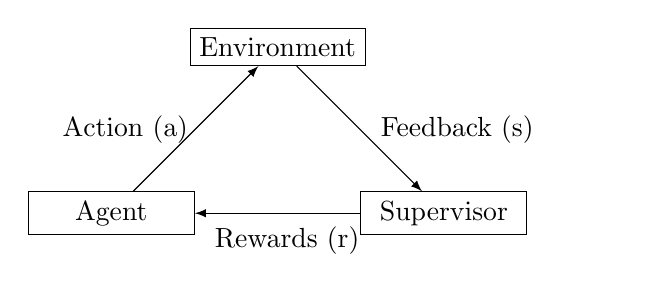
\begin{tikzpicture}[>=latex,every node/.style={rectangle,minimum width={6em},node distance=8.5em}]
			\node [draw](a) {Environment};
			\node [draw,below left of=a] (b) {Agent};
			\node [draw,below right of=a] (c) {Supervisor};
			\node [text width=3cm] at (8em, -3em) {Feedback (s)};
			\node [text width=3cm] at (-3.5em, -3em) {Action (a)};
			\node [text width=3cm] at (2em, -7em) {Rewards (r)};
			\draw [->] (b) -- (a);
			\draw [->] (a) -- (c);
			\draw [->] (c) -- (b);
			
			\end{tikzpicture}
			\caption{Diagram of reinforcement learning scheme.}
		\end{center}
		\label{diagram}
	\end{figure}
	
	According to \cite{Sutton:1998} a typical reinforcement learn model consists of:
	
	\begin{itemize}
		\item a discrete set of environment states, $s$;
		\item a discrete set of agent actions, $a$; and
		\item a set of scalar reinforcement signals; typically {0; 1}, or the real numbers.
	\end{itemize}
	
	For this work, we use an particular approach of reinforcement learning, known as learning automata. Wu \& Liao \cite{Wu:2013} proposed learning automata in order to solve complex function optimisation problems, and named his model as Function Optimisation by Learning Automata (FOLA). These authors demonstrate that learning automata improves the optimization performance in terms of its convergence rate and accuracy, requiring less computation time in order to obtain a more accurate solutions, especially for high-dimensional functions.
	
	In this approach, the automata updates the action probabilities according to the responses of the environment. Specifically, for this project, FALA (\emph{finite action-set learning automata}) will be used \cite{Narendra:1989}. Given the state-set $S$, FALA can be described as:
	
	\begin{equation}
	\label{eq: FALA}
	\Gamma = (A,R,\tau,\overline{P}(t))
	\end{equation}
	where $A = \{a_0,a_1,a_2,...,a_n\}$ is the finite action-set, $R$ is the reinforcement signal-set, $\tau$ the learning scheme and $\overline{P}(t)$ is the vector or probabilities. In this case, $\overline{P}_{i}(t)$ is the probability of an action $a_i$ to be chosen at the time $t$. Notice that, I assume that $\overline{P}_{i}(t) \geq 0$ and $\sum_{i=0}^{n} \overline{P}_{i}(t) = 1$.
	
	Thus, the vector of probabilities $\overline{P}(t)$ is updated according as following learning algorithm:
	
	\begin{equation}
	\label{eq: updateFALA}
	\overline{P}_{(t+1)} = \tau(\overline{P}_{(t)},a(t),R(t))
	\end{equation}
	This means that the updated probability $\overline{P}_{(t+1)}$ depends on the current vector of probabilities $\overline{P}_{(t)}$, the action $i$ chosen $a_{i}(t)$ and the reward $R$ at time $t$. Basically, the process is as follow: On every moment $t$, an action $a_{i}(t)$ is taken according to the vector of probabilities $\overline{P}_{(t)}$. The output is an reaction or a change of state to $S(t+1)$. Afterward, based on the state $S(t+1)$, the quality of the result is measured and the reward is calculated according to the parameters in the set $R$. In the end, the value of $R$ is used to update the vector of probabilities $\overline{P}_{(t+1)}$ \cite{Narendra:1989}. 
	
	\vspace{0.6cm}
	\section{Model} \label{model}

Usually, the components of the individual portfolio are given is often assumed in the literature of portfolio optimization problem \cite{Brandt2007}. Nonetheless, we highlight that our objective is to find out a subset of components, among a extensive list of securities, aiming to construct a portfolio. The model for the portfolio level of risk is:

\begin{equation}
\begin{aligned}
& \underset{\mathcal{W}}{\text{Min}}
& & \sigma = (\mathcal{W}' * \Sigma * \mathcal{W})^{0.5} \\
%& \text{subject to}
%& & \sum_{n=1}^{10} w_n = 1 \\
%&&& 0 =< w_n =<1.
\end{aligned}
\label{eq: portfolio_risk}
\end{equation}
where $\sigma$ is the level of risk, $\mathcal{W} = \{w_1, w_2, ..., w_{10}\}$ is the vector of weights and $\Sigma$ is the covariance matrix based on the historical returns of a given set of components. And the model for the portfolio Sharpe ratio is:

\begin{equation}
\begin{aligned}
& \underset{\mathcal{W}}{\text{Max}}
& & Sharpe= \frac{\mathcal{W}'E(Ret)}{\sigma} \\
%& \text{subject to}
%& & \sum_{n=1}^{10} w_n = 1 \\
%&&& 0 =< w_n =<1.
\end{aligned}
\label{eq: portfolio_sharpe}
\end{equation}
where $Sharpe$ is the Sharpe ratio, $E(Ret) = \{E(ret_1), E(ret_2), ... , E(ret_{10})\}$ is the vector of expected return. The constraints for $w$ is at both of the (\ref{eq: portfolio_risk}) and (\ref{eq: portfolio_sharpe}) are $\sum_{n=1}^{10} w_n = 1$ and $0 =< w_n =<1$.

For the purpose of this work, our model is divided in two steps. Firstly, we employ learning automata to select the components of an individual portfolio. And secondly, we use a traditional solver in order to find the vector of weights that optimize this portfolio.

For example, let's use learning automata to find out the components of an individual portfolio that has the most accurate minimal risk. In order to do so, our list of variables is composed as below (see details in Section \ref{methodology}):
\begin{itemize}
\item $\mathcal{P}_t$ is vector of probabilities of each component to be selected at moment $t$.
\item action-set $\mathcal{A}$ is the list of 500 components of the S\&P 500 Index, $N=500$.
\item $\mathcal{A}_t = \{a^1_t,a^2_t,...,a^{10}_t\}$ is the list of ten stocks selected to risk optimization at moment $t$.
\item $\mathcal{A}^*_T$ is the list of ten stocks that belongs to the action-set $\mathcal{A}$ with the highest probabilities.
\item $\sigma^*_T$ is the optimal portfolio risk along of the algorithm.
\item $\sigma^*_t$ is the optimal portfolio risk at time $t$.
\item reinforcement signal $\mathcal{R}$ is the set signal.
\item learning scheme $\tau$ is the function that update the vector of probabilities.
\item $\mathcal{W}$ is the vector of portfolio weights.
\end{itemize}

\begin{figure}[hbt]
\small
\setstretch{1.25}
\begin{algorithmic}[1]
\Require $\mathcal{A}$
\Ensure $\sigma^*_T$ , $\mathcal{A}^*_T$ , $\mathcal{W}^*_T $
\For {$n=1$ to 30} \Comment{Number of runs}
	\State $\sigma^*_T \gets 10 $ \Comment{Initiate optimal global risk $\sigma^*_T$ }
    \State $\mathcal{P}_t(\mathcal{A})  \gets 1/N$\Comment{Initiate vector of probabilities $\mathcal{P}_t(\mathcal{A})$}
  \While{$\sum_1^{10}{\mathcal{P}_t(\mathcal{A}^*_T)}<0.99$ and $t<1000$}  \label{alg:while}
	\State $\mathcal{A}_t \gets \mathcal{P}_t(\mathcal{A})$\Comment{ Select ten components randomly}
	\State $\sigma^*_t \gets SD(\mathcal{A}_t)$\Comment{ Optimal risk by using (\ref{eq: portfolio_risk})}
	\If{$\sigma^*_t<\sigma^*_T$} \label{alg:receivedSignalV}%\COMMENT{from $v$}
		\State $\sigma^*_T\gets\sigma^*_t$
        \State $\mathcal{A}^*_T \gets \mathcal{A}_t$
        \State $\mathcal{W}^*_T \gets \mathcal{W}_t$
	\EndIf
	\State $\mathcal{R}(\mathcal{A}^*) \gets 0.001$ \Comment{Reinforcement signal}
	\State $\mathcal{P}_{t+1}(\mathcal{A}) \gets \mathcal{P}_t(\mathcal{A}) + \mathcal{R}(\mathcal{A}^*_T)$ \Comment{Transition function}
	\State $\mathcal{P}_{t+1}(\mathcal{A}) \gets \mathcal{P}_{t+1}(\mathcal{A})/ \sum \mathcal{P}_{t+1}(\mathcal{A}) $. \Comment{Normalization}
    \State $t  \gets t+1$
  \EndWhile
\EndFor
\end{algorithmic}
\caption{Application of learning automata to select the portfolio components in terms of risk}
\label{alg: ls}
\end{figure}

Figure \ref{alg: ls} shows the algorithm based on learning automata to select the components of an individual portfolio in terms of risk $\sigma$. From this figure, notice the following. Firstly, the algorithm will be terminated whether the sum of the top-ten probabilities of a component to be selected $\sum_1^{10}{\mathcal{P}_t(\mathcal{A}^*_T)}<0.99$ is superior to the threshold of $0.99$, or the amount of loops $t$ is equal to 1000. Secondly, the components that results in the lowest level of risk $\sigma^*_T$ of this algorithm is updated whether the minimal risk of the portfolio at algorithm $\sigma^*_t$ is inferior to this value. Thirdly, the probability of the components that shows the lowest level of risk along of the algorithm process $\sigma^*_T$ is updated according to the reinforcement signal $\mathcal{R}(\mathcal{A}^*)=0.001$. Finally, the transition function is updated according the reinforcement signal received $\mathcal{P}_{t+1}(\mathcal{A}) \gets \mathcal{P}_t(\mathcal{A}) + \mathcal{R}(\mathcal{A}^*_T)$.
		\section{Data and Empirical Results}
	
	The study is based on a	broad intradaily financial dataset comprising 41 assets listed on the B3 from 2009 to 2017
	
	Our empirical application uses B3's stock returns
	
	In our empirical analysis we have used high frequency data on transaction prices for assets listed on the B3. The sample period ran from December 18, 2009 to February 17, 2017, delivering 1761 distinct days. We have used functions from the “GetHFData” R package by Perlin and Ramos (2016) in different stages of the data cleaning process. In the first step, we discarded any record with a timestamp outside the regular marketing opening hours. Throughout our sample, the official B3 trading day have changed ten times, being the opening time at 10 a.m. or at 11 a.m. and the closing time between 16:55 and 17:55. On holy Wednesday the stock exchange operates half day. Those days were discarded in order to avoid outliers. The same was done on dates in which there were
	delays due to technical failure or matches of the Brazil national team in the 2014 FIFA World Cup, resulting in the elimination of 13 observations. Canceled trades were also deleted. The ticker symbols, names and sector for each of the assets are provided in the appendix (table A.1).
	We adjusted our historical price data to remove gaps caused by stock splits and reverse stock splits in order to prevent misleading signals. Other adjustments were made to remove smaller	gaps caused by different types of corporate actions, such as dividends, bonus issues of shares, rights issues of shares, interest on equity and spinoffs. Such adjustments ensure that all the resulting price movements are caused solely by market forces.
	
	The daily closing price was used to compute squared close to close log returns. They were not part of our intradaily data series, since they are defined by
	an auction, after the regular trading hours.
	
	Beyond this	reason, our choice of sampling frequency is related to the liquidity level of the shares listed in B3.
	
%	B3. (n.d.). Listed Companies. Available at: http://www.bmfbovespa.com.br/en_us/products/listedequities-
%	and-derivatives/equities/listed-companies.htm. Accessed: 2017-06-01.
	
	Our data set consists of daily data of adjusted closing prices of all stocks that belongs to the S\&P 500 market index from July 1990 to December 2015, a time period that covers several market upturns and downturns, as well as relatively calm and volatile periods. We obtain adjusted closing prices from Bloomberg, whereas returns on the Fama and French factors are obtained from French's website\footnote{\url{http://mba.tuck.dartmouth.edu/pages/faculty/ken.french/Data_Library/det_st_rev_factor_daily.html}}. The data set spans 6,426 days and includes a total of 1100 stocks over all periods. Only stocks that are listed during the formation period are included in the analysis, \emph{i.e.}, around 500 stocks in each trading period. We assume that all trades occur at the closing price of that day.
	
	
	Using data from the Center for Research in Security Prices (CRSP) from 1980 to 2006, \citet*{french2008} estimates that the cost of active investing, including total commissions, bid-ask spreads, and other cost investors pay for trading services, has dropped from 146 basis points in 1980 to 11 basis points in 2006. Considering the US stock live trades on the Nyse-Amex between August 1998 and September 2013 for a large institucional investor, \citet*{fim15} estimate that the average trading costs for market impact (MI) and implementation shortfall methodology (IS) are 8.81 and 9.13 basis points, respectively, while the median trading costs are 6.24 and 7.63 basis points, respectively. \citet{avellaneda2010, stubinger2016,liu2017,stubinger2018} assume transaction costs of 5 basis points per share half-turn, thus 10 basis points for the round-trip transaction cost. Following these studies, we assume trading costs of 0.10\% (10 basis points) and 0.20\% (20 basis points) per round-trip pair trade.
	

	
	\vspace{0.3cm}
	
	
	\subsection{Profitability of the Strategies}
	
First, we provide multiple boxplots in Figures \ref{fig:Figure1} and \ref{fig:Figure2} to analyze the sensitivity of the annualized excess returns (Figure \ref{fig:Figure1}) and annualized Sharpe ratios (Figure \ref{fig:Figure2}) when the opening thresholds $\Delta_{1}$ and $\Delta_{2}$ are changed to top 5, 10, 15, 20, 25, 30 and 35 pairs for each of the strategies from 1991/2-2015 on commited capital and on fully invested capital after costs (10 bps)\footnote{The numerical experiments show that the relative performances out-of-sample stay very similar when we consider 20 bps. Since the results are very much alike they are not presented here and are available under request. Hereafter, we consider 10 basis points as transaction costs to report results for the remainder of this paper.}. Pairs are formed based on the smallest sum of squared deviations. The last boxplot (from left to right) shows the performance for the distance strategy (2.0$\sigma$), while the others report the outcomes using multiple opening trigger points for the cumulative mispricing indexes $M_{1,t}$ and $M_{2,t}$ (one above 0.05, 0.1, 0.15, 0.2, 0.25, 0.3, 0.35, 0.4, and 0.55 and the other one below their negative counterparts). Based on these outcomes we perform the subsequent analyses considering 0.2 and -0.2 as the opening thresholds for the mixed copula strategy.

\begin{figure}[!ht]
	\centering
	%\includegraphics[scale=0.26]{fig26.pdf}
	%\includegraphics[width=\linewidth,height=7.5cm]{fig26.pdf}
	%		\resizebox{\linewidth}{!}{\input{Figure1.tex}}
	%		\captionsetup{justification=raggedright,
	%		singlelinecheck=false
	%	}
	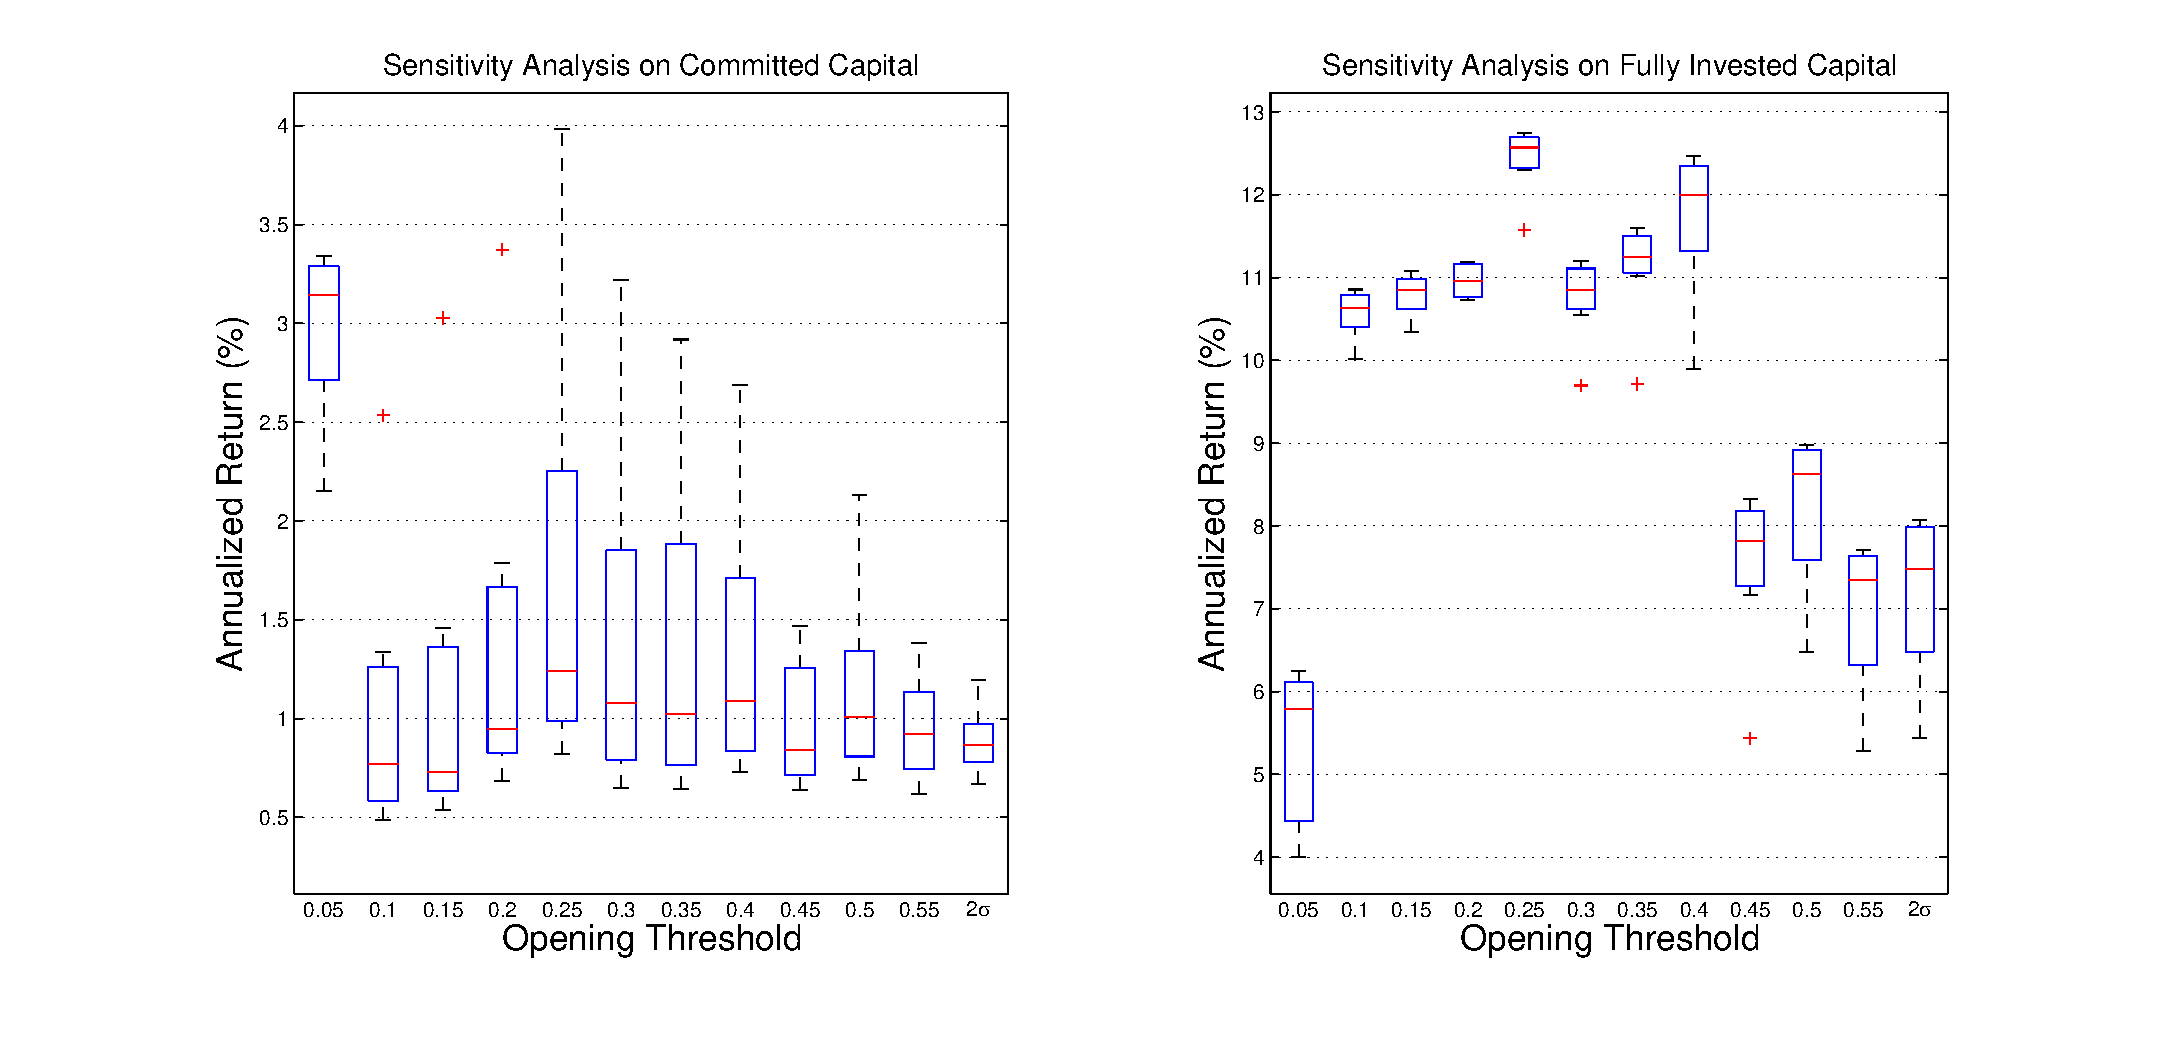
\includegraphics[width=\linewidth]{Figure1.eps}
	\captionsetup{justification=raggedright,
		singlelinecheck=false
	}
	\caption{\textbf{Annualized returns of pairs trading strategies after costs on committed and fully invested capital}}
	\caption*{\scriptsize These boxplots show annualized returns on committed (left) and fully invested (right) capital after transaction cost to different opening thresholds from July 1991 to December 2015 for Top 5 to Top 35 pairs. Pairs are formed based on the smallest sum of squared deviations.}
	\label{fig:Figure1}
\end{figure}

\begin{figure}[!ht]
	\centering
%	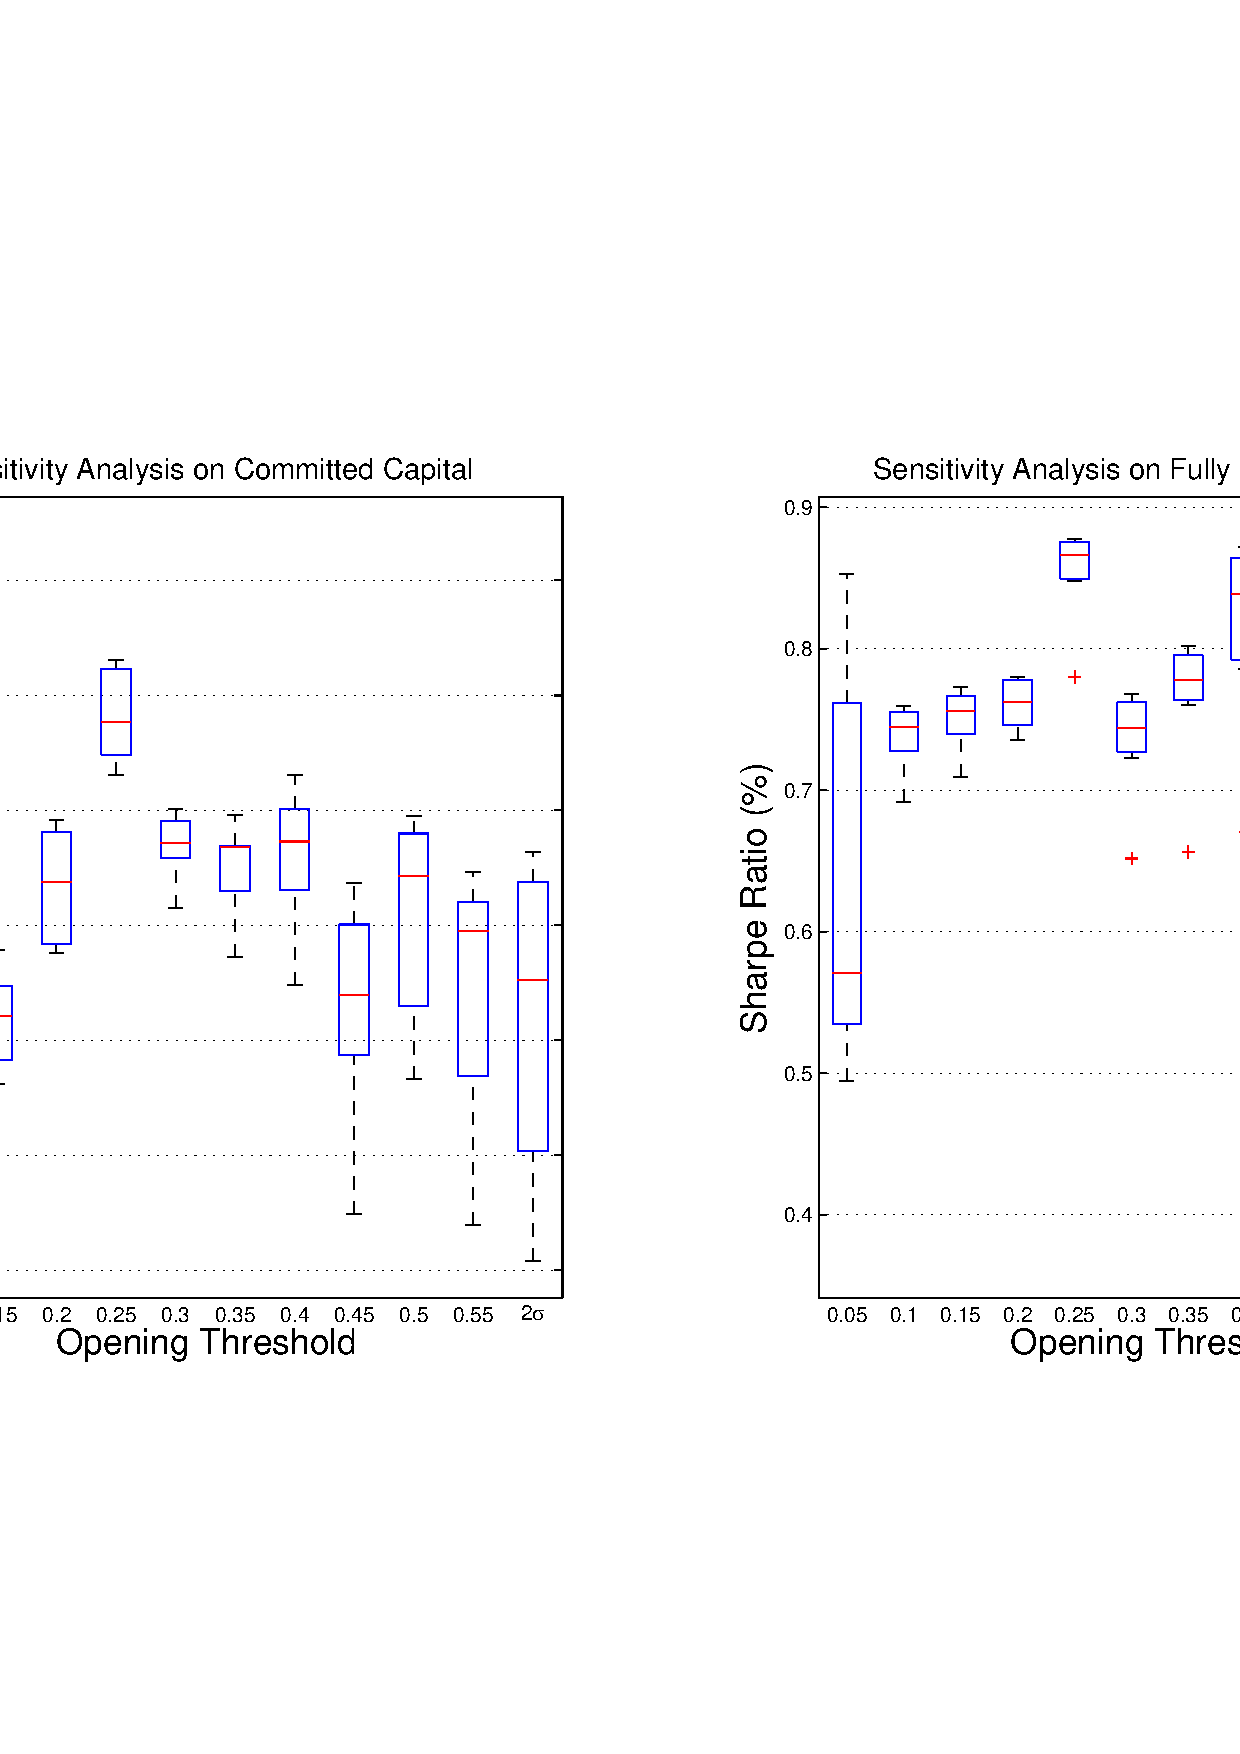
\includegraphics[width=\linewidth,height=7.5cm]{Figure2.pdf}
%	\resizebox{\linewidth}{!}{\input{Figure2.tex}}
%	\captionsetup{justification=raggedright,
%		singlelinecheck=false
%	}
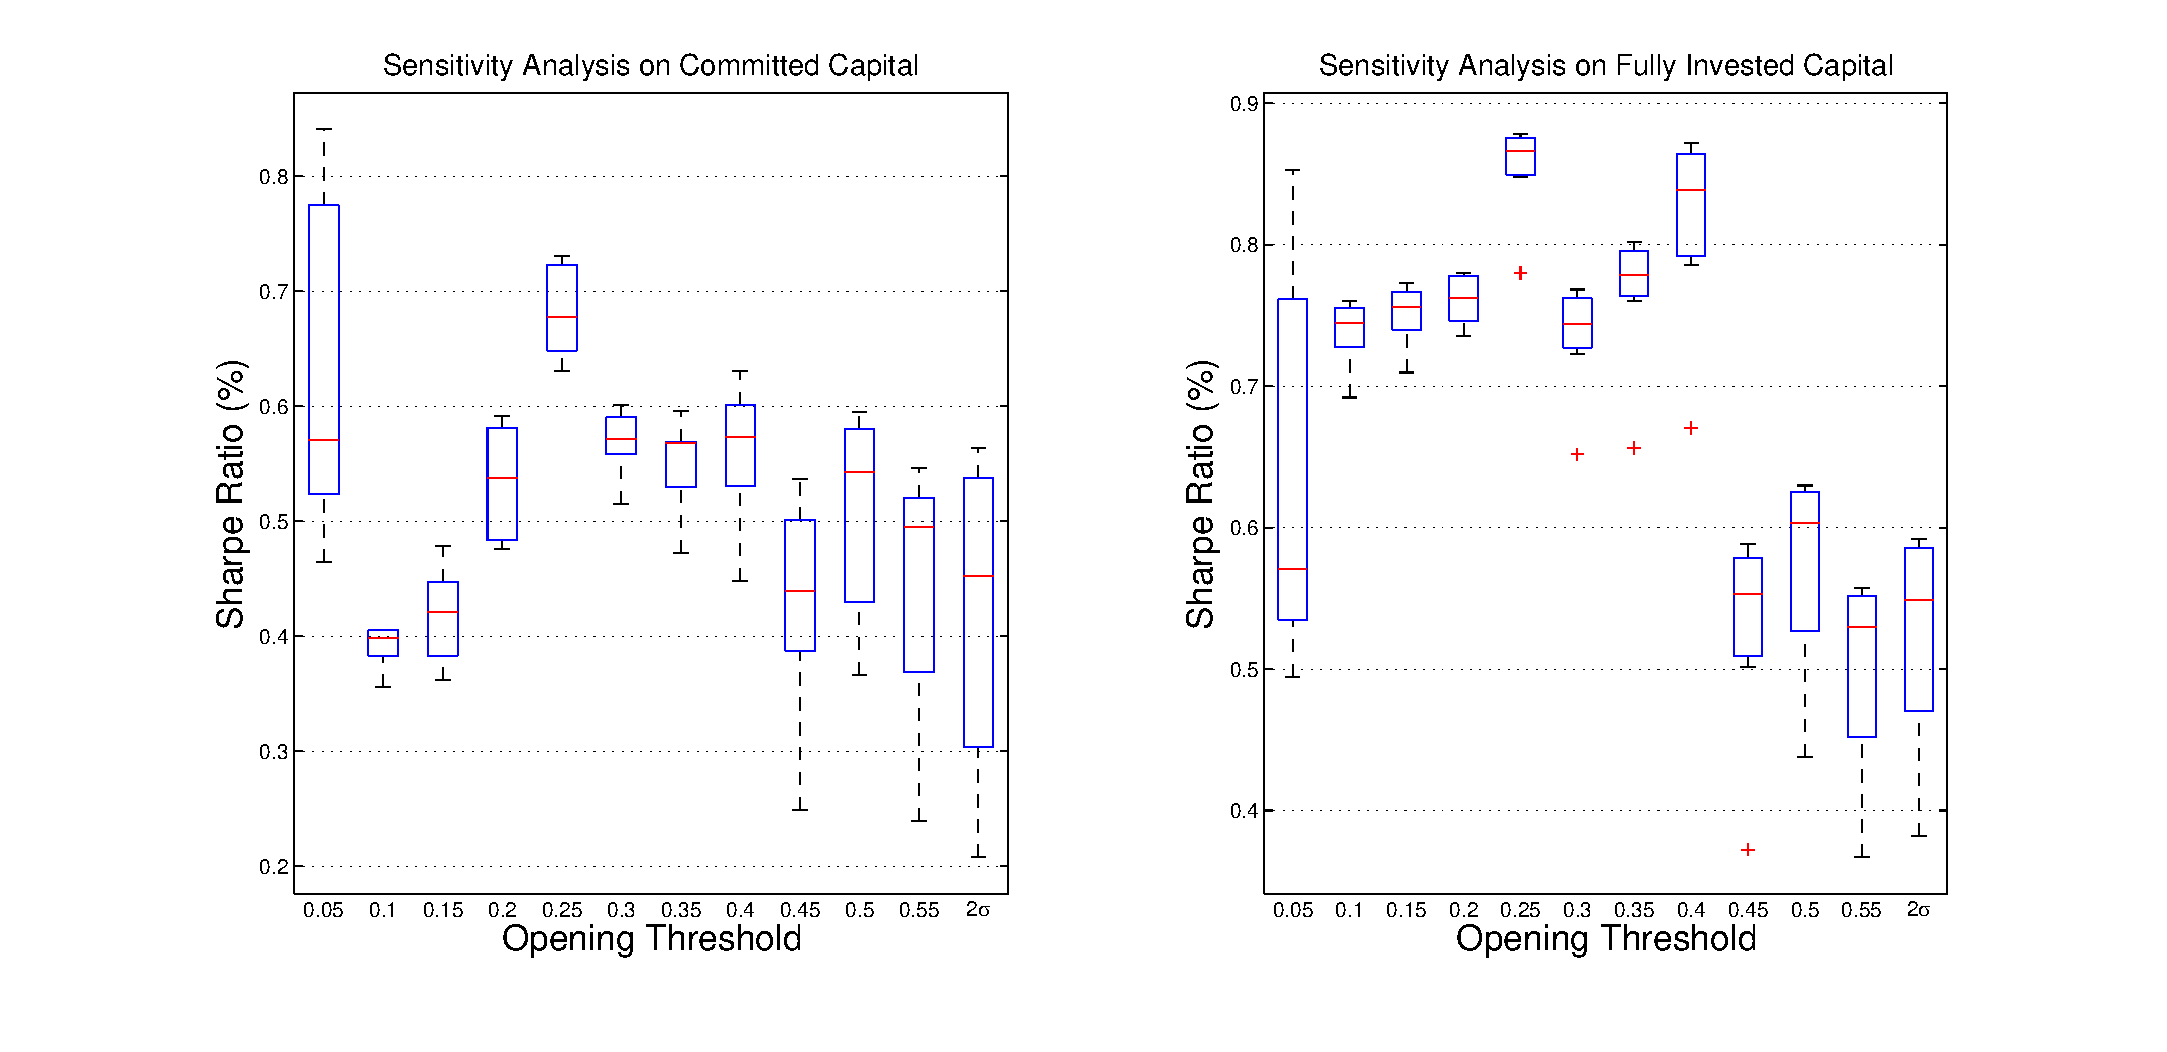
\includegraphics[width=\linewidth]{Figure2.eps}
\captionsetup{justification=raggedright,
	singlelinecheck=false
}
\caption{\textbf {Sharpe ratio of pairs trading strategies after costs on committed and fully invested capital}}
\begin{quote} {\scriptsize These boxplots show Sharpe ratios on committed (left) and fully invested (right) capital after transaction cost to different opening thresholds from July 1991 to December 2015 for Top 5 to Top 35 pairs. Pairs are formed based on the smallest sum of squared deviations.}\end{quote}
\label{fig:Figure2}
\end{figure}

Table \ref{tab:table101} reports annualized mean excess returns, annualized Sharpe and Sortino ratios, \citet*{nw87} adjusted t-statistics, share of negative observations, the maximum drawdown in terms of maximum percentage drop between two consecutive days (MDD1) and between two days within a period of maximum six months (MDD2), annualized standard deviation, minimum and maximum daily return for both strategies from 1991/2-2015, for Top 5 (Panel A), Top 20 (Panel B), and Top 35 (panel C) pairs after costs (10 bps)\footnote{The outcomes are also robust for the other number of pairs considered. Since the results are very much alike they are not presented here and are available under request.}. Furthermore, Section 1 shows the return on Committed Capital and Section 2 on Fully Invested Capital. %Panel A lists the results after transaction costs and Panel B before transaction costs. 	
	
By analyzing Table \ref{tab:table101}, it is possible to observe a series of important facts. First, note that the copula-based pairs strategy outperforms the distance method for Top 5 pairs and committed capital. The mixed copula strategy yields the highest average excess returns (3.98\%), the lowest annualized standard deviation (6.31\%) and reaches a Sharpe ratio of 0.63 after costs, over twice as much as what we get from investing in the tradicional distance method. The Sortino ratio confirms that the mixed copula model offers better risk-adjusted returns. The statistics also indicate that the mixed copula model delivers the highest t-statistics (statistically significant at 1\% and economically large as well) and a lower probability of a negative trade, where the share of days with negative returns (41.79\%) is consistently smaller than the market performance (47.45\% of negative returns over the period). Furthermore, the summary statistics also show that mixed copula method offers better hedges against losses than the distance strategy for Top 5 pairs on committed capital when considering the downside risk statistics MDD1 and MDD2. We find that the number of tradeable signals along the competitive strategies is only equiparable in this study for the case of Top 5 pairs. We will explore this point further in the next subsection.

 The listed results for Top 20 and Top 35 pairs on committed capital show that the distance strategy is more profitable than the mixed copula method, although the Sharpe ratios are similar, indicating that returns are alike when we take into account the risks taken. All profits are statistically significant at 1\%. Overall, the copula method is again a less risky strategy regarding the drawdown measures.

\begin{threeparttable}[H]
	\centering \scriptsize
	\caption{Excess returns of pairs trading strategies on portfolios of Top 5, 20 and 35 pairs after costs.}
	\begin{tabularx}{\textwidth}{@{\extracolsep{\fill}}lllllll@{}}
		\toprule
		& \multicolumn{3}{c}{Distance} & \multicolumn{3}{c}{Mixed Copula} \\\cmidrule{2-4} \cmidrule{5-7}
		& Top 5 & Top 20 & Top 35 & Top 5 & Top 20 & Top 35 \\
		\midrule
		& \multicolumn{6}{c}{\textbf{Section 1: Return on Committed Capital}} \\
		& \multicolumn{6}{c}{\textit {Panel A: after transaction costs}} \\
		Annualized Mean Return (\%) & 2.60  & $3.14^{*}$  & $3.12^{***}$  & 3.98  & 1.24  & 0.82 \\
		Sharpe ratio & 0.31  & 0.65  & 0.77  & 0.63  & 0.64  & 0.73 \\
		Sortino Ratio & 0.58  & 1.13  & 1.36  & 1.08  & 1.04  & 1.19 \\
		t-stat & $1.86^{*}$  & $3.31^{***}$  & $3.92^{***}$  & $3.49^{***}$  & $3.52^{***}$  & $3.95^{***}$ \\
		\% of negative trades & 46.98 & 48.06 & 47.97 & 41.79 & 41.33 & 41.31 \\
		MDD1  & 6.73  & 3.88  & 2.70  & 4.36  & 2.07  & 1.18 \\
		MDD2  & 19.62 & 9.69  & 7.52  & 9.29  & 3.43  & 1.98 \\
		Annualized Std. Dev. (\%) & 8.25  & 4.87  & 4.06  & $6.31^{***}$  & $1.93^{***}$  & $1.12^{***}$ \\
%		Skewness & 0.25  & 0.32  & 0.28  & -0.04 & -0.25 & -0.01 \\
%		Kurtosis & 9.17  & 9.76  & 5.46  & 10.32 & 11.98 & 12.93 \\
		Minimum Daily Return (\%) & -4.43 & -2.76 & -1.50 & -4.16 & -1.47 & -0.84 \\
		Maximum Daily Return (\%) & 5.39  & 2.81  & 1.76  & 3.47  & 0.87  & 0.68 \\
		\midrule
		& \multicolumn{6}{c}{\textit {Panel B: before transaction costs}} \\
		Annualized Mean Return (\%) & 2.90  & $3.43^{**}$  & $3.39^{***}$  & 4.29  & 1.40  & 0.93 \\
		Sharpe ratio & 0.35  & 0.70  & 0.83  & 0.68  & 0.73  & 0.83 \\
		Sortino Ratio & 0.64  & 1.23  & 1.48  & 1.16  & 1.18  & 1.36 \\
		t-stat & $2.04^{**}$  & $3.59^{***}$  & $4.25^{***}$  & $3.73^{***}$  & $3.95^{***}$  & $4.46^{***}$ \\
		\% of negative trades & 46.95 & 47.87 & 47.77 & 41.65 & 41.24 & 41.20 \\
		MDD1  & 6.73  & 3.89  & 2.69  & 4.36  & 2.07  & 1.18 \\
		MDD2  & 19.61 & 9.55  & 7.43  & 9.25  & 3.37  & 1.94 \\
		Annualized Std. Dev. (\%) & 8.27  & 4.88  & 4.07  & $6.33^{***}$  & $1.93^{***}$  & $1.13^{***}$ \\
%		Skewness & 0.26  & 0.33  & 0.29  & -0.04 & -0.23 & 0.07 \\
%		Kurtosis & 9.19  & 9.78  & 5.46  & 10.31 & 11.91 & 12.96 \\
		Minimum Daily Return (\%) & -4.43 & -2.77 & -1.50 & -4.16 & -1.47 & -0.84 \\
		Maximum Daily Return (\%) & 5.41  & 2.81  & 1.77  & 3.47  & 0.87  & 0.68 \\
		\midrule
& \multicolumn{6}{c}{\textbf{Section 2: Return on Fully Invested Capital}} \\
& \multicolumn{6}{c}{\textit {Panel A: after transaction costs}} \\
		Annualized Mean Return (\%) & 4.01  & 6.07  & 5.76  & $11.58^{*}$ & $12.30^{**}$ & $12.73^{**}$ \\
		Sharpe ratio & 0.28  & 0.66  & 0.76  & $0.78^{**}$  & 0.85  & 0.88 \\
		Sortino Ratio & 0.57  & 1.19  & 1.38  & 1.43  & 1.54  & 1.59 \\
		t-stat & $1.81^{*}$  & $3.55^{***}$  & $4.05^{***}$  & $4.26^{***}$  & $4.60^{***}$  & $4.73^{***}$ \\
		\% of negative trades & 46.98 & 48.06 & 47.97 & 41.79 & 41.31 & 41.28 \\
		MDD1  & 8.70  & 5.43  & 4.24  & 9.00  & 9.00  & 9.00 \\
		MDD2  & 38.36 & 20.03 & 15.07 & 25.68 & 25.68 & 25.68 \\
		Annualized Std. Dev. (\%) & 14.51 & $9.20^{***}$  & $7.57^{***}$  & 14.84 & 14.51 & 14.51 \\
%		Skewness & 0.26  & 0.04  & 0.19  & 0.15  & 0.14  & 0.15 \\
%		Kurtosis & 11.27 & 5.85  & 4.04  & 11.07 & 12.28 & 12.35 \\
		Minimum Daily Return (\%) & -8.34 & -4.71 & -3.10 & -10.19 & -10.19 & -10.19 \\
		Maximum Daily Return (\%) & 10.07 & 3.74  & 3.17  & 10.16 & 10.16 & 10.16 \\
		\midrule
& \multicolumn{6}{c}{\textit {Panel B: before transaction costs}} \\ 
		Annualized Mean Return (\%) & 4.49  & 6.56  & 6.24  & $12.30^{**}$ & $13.10^{**}$ & $13.53^{**}$ \\
		Sharpe ratio & 0.31  & 0.71  & 0.82  & $0.82^{**}$  & 0.90  & 0.93 \\
		Sortino Ratio & 0.63  & 1.28  & 1.49  & 1.51  & 1.62  & 1.68 \\
		t-stat & $1.98^{**}$  & $3.81^{***}$  & $4.35^{***}$  & $4.48^{***}$  & $4.84^{***}$  & $4.98^{***}$ \\
		\% of negative trades & 46.95 & 47.87 & 47.77 & 41.65 & 41.24 & 41.20 \\
		MDD1  & 8.71  & 5.43  & 4.23  & 9.00  & 9.00  & 9.00 \\
		MDD2  & 38.30 & 19.89 & 14.93 & 25.60 & 25.60 & 25.60 \\
		Annualized Std. Dev. (\%) & 14.56 & $9.23^{***}$  & $7.60^{***}$  & 14.91 & 14.59 & 0.15 \\
%		Skewness & 0.27  & 0.04  & 0.19  & 0.16  & 0.14  & 0.15 \\
%		Kurtosis & 11.25 & 5.86  & 4.04  & 11.03 & 12.22 & 12.29 \\
		Minimum Daily Return (\%) & -8.34 & -4.71 & -3.10 & -10.19 & -10.19 & -10.19 \\
		Maximum Daily Return (\%) & 10.07 & 3.75  & 3.18  & 10.16 & 10.16 & 10.16 \\
		\bottomrule
\end{tabularx}
\begin{tablenotes}
\item \textit{Note:} \scriptsize Summary statistics of the annualized excess returns, standard devations, Sharpe and Sortino ratios on portfolios of top 5, 20 and 35 pairs between July 1991 and December 2015 (6,173 observations). \textcolor{blue} {Pairs are formed based on the smallest sum of squared deviations}. The t-statistics are computed using Newey-West standard errors with a six-lag correction. The columns labeled MDD1 and MDD2 compute the largest drawdown in terms of maximum percentage drop between two consecutive days and between two days within a period of maximum six months, respectively.
\item \footnotesize $^{\ast\ast\ast}$, $^{\ast\ast}$, $^{\ast}$  significant at 1\%, 5\% and 10\% levels, respectively.
%\item \footnotesize The symbol labels (>) and (<) indicate that the null hypothesis represented in (\ref{eq:eq153}) is rejected in favor of the alternative and that the average excess returns, standard deviation, and Sharpe ratio of the mixed copula strategy are found greater (>) or lower (<) than the average excess returns, standard deviation, and the Sharpe ratio of the distance strategy, respectively.
\end{tablenotes}
\label{tab:table101}
\end{threeparttable}


\vspace{0.6cm}

%albeit with higher volatility.
Section 2 of Table \ref{tab:table101} shows results on fully invested capital scheme. We can note that this approach yields a higher Sharpe of 0.78 and Sortino ratio for the copula-based strategy and the excess return of the portfolio averaged 11.58\% a year (almost three times as large as the return of the committed capital approach), with large and significant Newey-West adjusted t-statistic of 4.26 for Top 5 pairs after costs. Apart from being a more volatile strategy, the mixed copula method consistently outperforms the distance strategy for all pairs considered.

Figure \ref{fig:Figure3} shows cumulative excess returns through the full dataset for both strategies for Top 5 (top), Top 20 (center) and Top 35 (bottom) pairs. The left panels display cumulative returns on committed capital, whereas the right panels on fully invested capital. The patterns found in the figure strengthen the mean returns and t-statistics displayed in Table \ref{tab:table101}. It should be noted that the mixed copula strategy shows a superior out-of-sample performance relative to the distance approach after the subprime mortgage crisis, especially after 2010 for Top 5 pairs (when the number of trades is comparable) on committed capital. 

\begin{figure}[!ht]
	\centering
	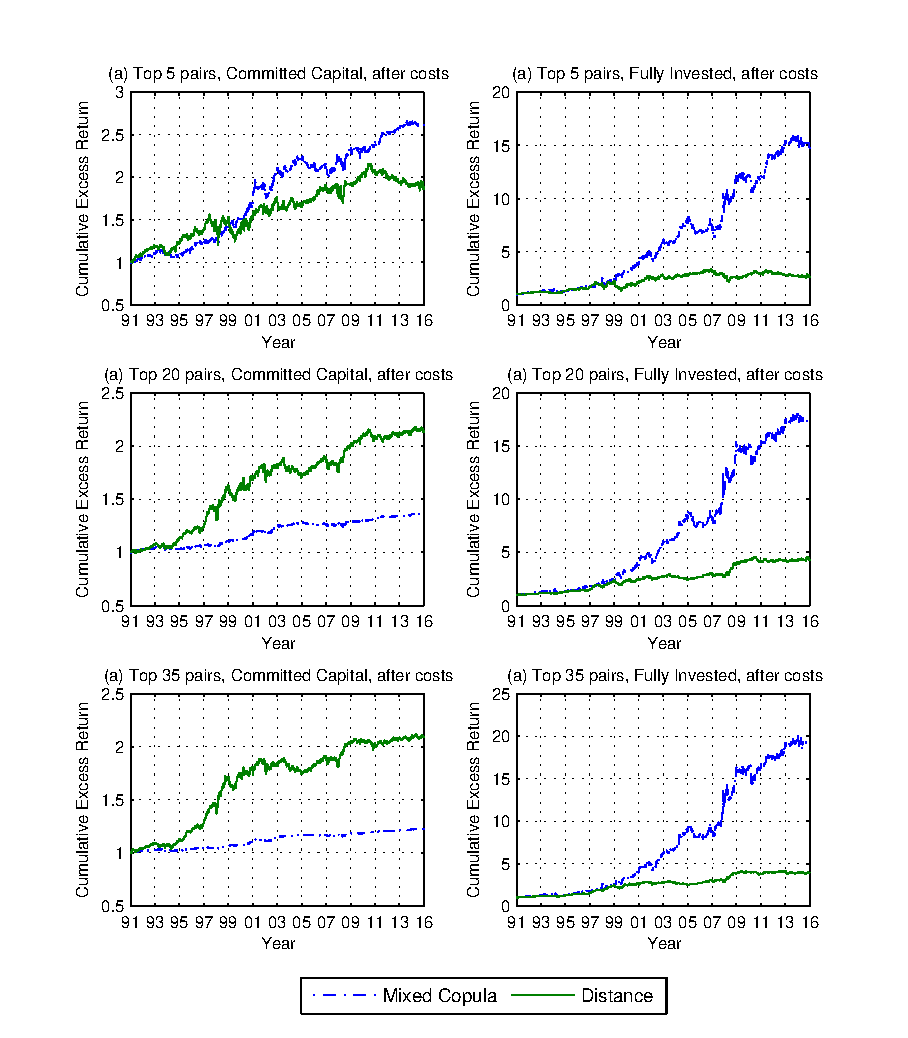
\includegraphics[width=\linewidth]{Figure3.eps}
	\captionsetup{justification=raggedright,
		singlelinecheck=false
	}
	\caption{\textbf{Cumulative excess returns of pairs trading strategies after costs}}
	\caption*{\scriptsize This figure shows how an investment of \$1 evolves from July 1991 to December 2015 for each of the strategies.}
	\label{fig:Figure3}
\end{figure}

Figure \ref{fig:Figure4} shows five-year rolling window Sharpe ratio after costs. The figure reveals mixed results over the long-term period. However, when the number of tradeable signals is similar (Top 5 pairs), the copula-based approach yields the highest five-year Sharpe ratio (up to 1.41) on committed capital in 68.94\% of the days. In 26.22\% of the days over the period the copula method delivers a rolling Sharpe ratio above 1, whereas the distance strategy never attains 1. In fact, the distance approach produces a five-year Sharpe ratio above 0.5 (and most often below zero after 2014) in only 25.4\% of the full period, indicating that the strategy does not reward the risk taken.

For Top 20 and Top 35 pairs on committed capital the strategies show a more competitive pattern. The distance approach presents a greater rolling window Sharpe ratio in 53.37\% and 50.99\% of the days for Top 20 and Top 35 pairs, respectively. However, as we will explore further, the distance approach is a more volatile strategy, identifying a greater number of trading opportunities (more opportunities to make profit) than the copula approach, making the comparison less reliable for a larger number of pairs. The 5-year Sharpe ratios for distance and mixed copula methods are greater than one in 24.97\% and 24.04\% for Top 20 pairs, and 31.92\% and 30.33\% for Top 35 pairs, respectively.

For fully invested weighting scheme the mixed copula approach achieves the highest five-year risk-adjusted statistic over the long-term period in 88.5\%, 69.14\% and 61.8\% of the data sample for Top 5, Top 20 and Top 35 pairs, respectively.


\begin{figure}[!ht]
\centering
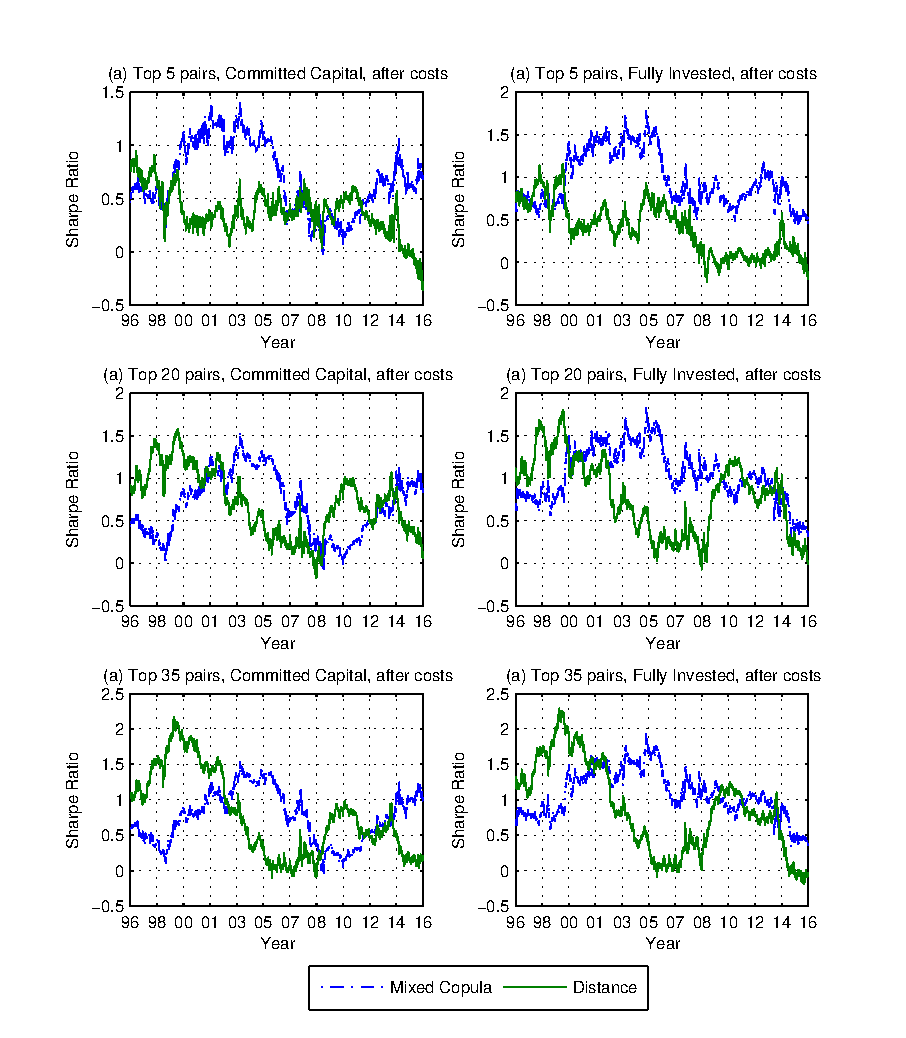
\includegraphics[width=\linewidth]{Figure4.eps}
\captionsetup{justification=raggedright,
	singlelinecheck=false
}
\caption{\textbf{Five-year rolling window Sharpe ratio after costs}}
\caption*{\scriptsize This figure shows how the 5-year rolling window Sharpe ratio evolves from July 1996 to December 2015 for each of the strategies.}
\label{fig:Figure4}
\end{figure}

\vspace{0.6cm}

Figure \ref{fig:Figure5} shows the densities of the five-year Sharpe ratios after costs estimated by means of \citet*{sj1991} bandwidth. As one can see, the densities reinforce our findings in Figure \ref{fig:Figure4}, showing that the right-hand tail of the distribution of the copula-based strategy remains long for Top 5 pairs.


\begin{figure}[!ht]
	\centering
	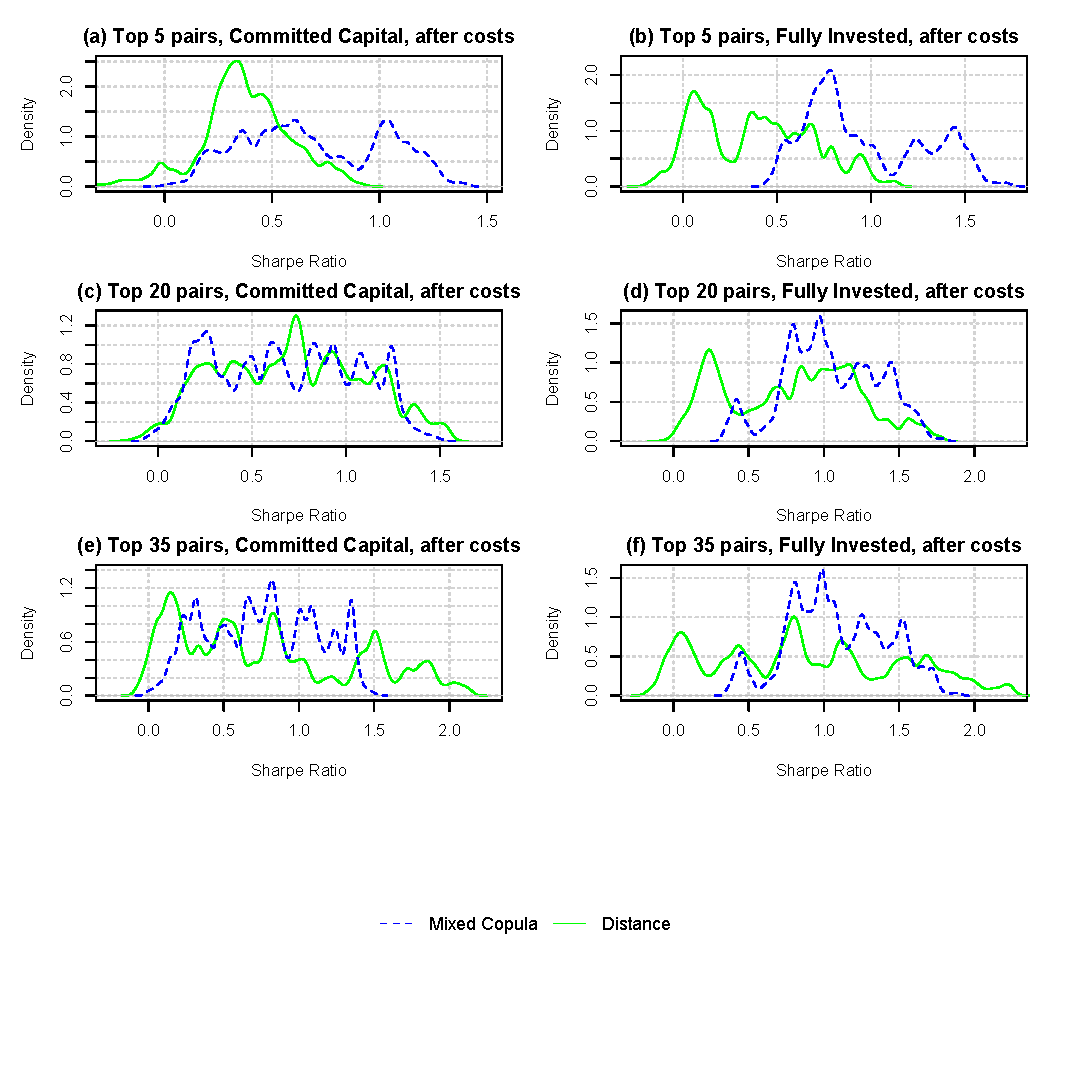
\includegraphics[width=\linewidth]{Figure5.eps}
	\captionsetup{justification=raggedright,
		singlelinecheck=false
	}
	\caption{\textbf{Kernel density estimation of 5-year rolling window Sharpe ratio after costs}}
	\caption*{\scriptsize  This figure shows how the 5-year rolling window Sharpe ratio densities evolve from July 1996 to December 2015 for each of the strategies with \citet*{sj1991}'s bandwidths.}
	\label{fig:Figure5}
\end{figure}

%Robustness checks of the performance of Excess Returns and Sharpe Ratios
One possible criticism might be that the conclusions are based on only one realization of the stochastic process of asset returns computed from the observed series of prices, since among thousands of different strategies is very likely that we find some that show superior performance in terms of excess returns or Sharpe Ratio for this specific realization. In order to mitigate data-snooping criticisms, we use the stationary bootstrap of \citet*{pr94} to compute the bootstrap p-values using the methodology proposed by \citet*{lw08}. 

%\footnote{It allows for weakly dependent correlation over time.}

%The bootstrap method is used to obtain the distribution of a null hypothesis. Here we want to investigate if the average excess return and the Sharpe Ratio of the Copula methods beat the reference (distance) strategies. To construct the distributions, we bootstrapped the original time series $B=10,000$ times. 
Our bootstrapped null distributions result from Theorem 2 of \citet*{pr94}. We select the optimal block length for the stationary bootstrap following \citet*{pw04}. As the optimal bootstrap block-length is different for each strategy, we average\footnote{We also use the optimal block size for each strategy. We find that the results are robust to the optimal block size, and therefore, we do not report them here.} the block-lengths found to proceed the comparisons between the mixed copula and the distance strategies.

To test the hypotheses that the average excess returns, standard deviations and Sharpe ratios of the copula-based strategy are equal to that of distance method, that is,
\begin{equation}
H_{0}:\mu_{c}=\mu_{d},  \ \
\ \  H_{0}:\sigma_{c}=\sigma_{d},
\ \ \textrm{and} \ \ H_{0}:\frac{\mu_{c}}{\sigma_{c}}=\frac{\mu_{d}}{\sigma_{d}},
\label{eq:eq153}
\end{equation}
we compute, following \citet*{davison1997}, a two-sided $p$-value using $B=10,000$ (stationary) bootstrap re-samples as follows:
\begin{equation}
p_{sboot}=
\begin{cases}
2\frac{\sum_{b=1}^{B}\mathbb{I}\{0< t^{\ast(b)}\}+1}{B+1}, &\text{if} ~~median\left\{ t^{\ast \left( 1\right) },...,t^{\ast \left( B\right)}\right\} > 0, \\
2\frac{\sum_{b=1}^{B}\mathbb{I}\{0\geq t^{\ast(b)}\}+1}{B+1}, &\text{otherwise},
\end{cases}
\label{eq:eq152}
\end{equation}
where $\mathbb{I}$ is the indicator function, $t^{\ast(b)}$ are the values in each block stationary bootstrap replication, and B denotes the number of bootstrap replications.

%Table \ref{tab:table101} report the bootstrap $p$-values for testing the null hypotheses represented by (\ref{eq:eq153}). We compare the copula method with each of the distance approaches (0.75 and 2.0 standard deviations) from 1991/2-2015 for all investment scenarios, \emph{i.e.}, without delay and waiting one-day period for the Top 5, Top 20, and Top 35 pairs, respectively, and before and after costs.

%The symbol labels (>) and (<) in Table \ref{tab:table101} indicate that the respective null hypothesis is rejected in favor of the alternative and that the average excess returns, standard deviation, and the Sharpe Ratio of the mixed copula approach are found greater (>) or lower (<) than their respective counterparts from the distance method.

Overall, these results reinforce the ones previously obtained. As it can be observed, the distance approach is more profitable than the copula method, at least at 10\%, for Top 20 and Top 35 pairs on committed capital. On the other hand, the copula approach significantly outperforms the distance strategy in terms of mean excess returns and in risk-adjusted returns when the number of tradeable signals is comparable (Top 5 pairs) on fully invested weighting structure.


\vspace{1.0cm}


	
	\subsection{Trading statistics}
	
	Table \ref{tab:table102} reports trading statistics. Panel A, B and C report results for Top 5, Top 20 and Top 35 pairs, respectively. The average price deviation trigger for opening pairs is listed in the first row of each panel. We can observe that, in average, we initiate the positions before when using the distance approach. The positions are initiated when prices have diverged by 5.94\%, 6.81\%, and 7.29\% for Top 5, Top 20, and Top 35 pairs, respectively. Similar to \citet*{ggr06}, the trigger spread increases with the number of pairs for all approaches\footnote{\citet*{ggr06} explains that the standard deviation of the prices increases as the proximity of the securities in price space decreases, thus increasing the trigger spreads.}.
	
	The table reveals that the average number of pairs traded per six-month period is only equiparable among the strategies for Top 5 pairs. For Top 20 and Top 35 pairs the total number of pairs opened is about 75\% and 138\% greater when starting positions based on the distance approach. This suggests that a two standard deviation trigger as opening criterion \citep{ggr06} is less conservative than the opening threshold suggested by \citet*{rf15} using the cumulative mispricing indexes $M_{1,t}$ and $M_{2,t}$. Thus, the distance approach will be able to identify more trading opportunities to profit making the comparison less meaningful, although in practice the benefits are partly offset by the trading costs.
	
	Finally, note that each pair is held open, in average, by 50.7 and 37.7 trading days (2.4 and 1.8 months) under the distance and copula approaches, respectively, for Top 5 pairs, which indicates that they are a medium-term investment under these strategies.
	
	\begin{threeparttable}[H]
		\centering \scriptsize
		\caption{Trading statistics.}
		\begin{tabularx}{\textwidth}{@{\extracolsep{\fill}}p{7cm}p{1cm}p{1cm}p{1cm}p{1cm}@{}}
			\toprule
			\multicolumn{1}{c}{Strategy} & Distance & Mixed Copula \\
			\midrule
			& \multicolumn{2}{c}{\textit{Panel A: Top 5}} \\
			& &  \\
			Average price deviation trigger for opening pairs & 0.0594 & 0.0665  \\
			Total number of pairs opened &  352   &  348   \\
			Average number of pairs traded per six-month period & 7.18 & 7.10    \\
			Average number of round-trip trades per pair & 1.44 & 1.42   \\
			~~Standard Deviation & 1.0128 & 1.33   \\
			Average time pairs are open in days &  50.70 &  37.70  \\
			~~Standard Deviation & 39.24 & 38.93    \\
			Median time pairs are open in days &  38.5  &  19          \\
			& &  \\
			& \multicolumn{2}{c}{\textit{Panel B: Top20}} \\
			& & \\
			Average price deviation trigger for opening pairs & 0.0681 & 0.0821    \\
			Total number of pairs opened &  1312  &  749     \\
			Average number of pairs traded per six-month period & 26.78 & 15.29   \\
			Average number of round-trip trades per pair & 1.34 & 0.76  \\
			~Standard Deviation & 0.99 & 0.99    \\
			Average time pairs are open in days & 51.65 & 23.60   \\
			~Standard Deviation & 39.62 & 32.90    \\
			Median time pairs are open in days & 41    & 9           \\
			& & \\
			& \multicolumn{2}{c}{\textit{Panel C: Top 35}} \\
			& & \\
			Average price deviation trigger for opening pairs & 0.0729 & 0.0893   \\
			Total number of pairs opened & 2238  & 941   \\
			Average number of pairs traded per six-month period & 45.68 & 19.20 \\
			Average number of round-trip trades per pair & 1.30 & 0.55   \\
			~Standard Deviation & 1.02 & 0.84   \\
			Average time pairs are open in days & 52.72 &  19.35   \\
			~Standard Deviation & 40.48 & 30.56  \\
			Median time pairs are open in days & 42    & 6           \\
	\bottomrule
\end{tabularx}%
\begin{tablenotes}
\item \textit{Note:} \footnotesize  Trading statistics for portfolio of top 5, 20 and 35 pairs between July 1991 and December 2015 (49 periods). \textcolor{blue} {Pairs are formed over a 12-month period according to a minimum-distance (sum of squared deviations) criterion} and then traded over the subsequent 6-month period. Average price deviation trigger for opening a pair is calculated as the price difference divided by the average of the prices.
\end{tablenotes}
\label{tab:table102}%
\end{threeparttable}%
	
	\vspace{1.0cm}
	
	
	
	\subsection{Regression on Fama-French asset pricing factors}
	
	In an attempt to understand the economic drivers behind our data as well as to evaluate whether pairs trading profitability is a compensation for risk, we regress daily excess returns onto various risk factors: daily \citet*{ff15}'s five research factors, the excess return on a broad market portfolio, ($R_{m} - R_{f}$), the difference between the return on a portfolio of small stocks and the return on a portfolio of large stocks ($SMB$, small minus big), the difference between the return on a portfolio of high book-to-market stocks and the return on a portfolio of low book-to-market stocks ($HML$, high minus low), the difference between the return of the most profitable stocks and the return of the least profitable stocks ($RMW$, robust minus weak), the difference between the return of stocks that invest conservatively and the return of stocks that invest aggressively ($CMA$, conservative minus aggressive) plus momentum (Mom),  short-term reversal (SRev), and long-term reversal (LRev) factors, \emph{i.e.},


	\begin{equation}
	\begin{aligned}
	R_{i,t}-R_{f,t}&=\alpha _{i}+\beta _{i}\left( R_{m,t}-R_{f,t}\right)+s_{i}SMB_{t}+h_{i}HML_{t}+r_{i}RMW_{t}\\
	&~+c_{i}CMA_{t}+m_{i}Mom_{t}+v_{i}SRev_{t}+l_{i}LRev_{t}+\varepsilon _{i,t},
	\end{aligned}
	\label{eq:eq101}
	\end{equation}
with $E(\varepsilon _{i,t})=0$, $Var(\varepsilon _{i,t})=\sigma_{\varepsilon _{i}}^{2}$ and $E(\varepsilon _{i,t}\varepsilon _{i,s})=0, t \neq s$, where $i$ and $t$ stands for portfolio and time index, respectively.
	
		All the data used to fit the above regressions are described in and obtained from Kenneth French’s data library\footnote{\url{http://http://mba.tuck.dartmouth.edu/pages/faculty/ken.french/data_library.html}}. We select the model in terms of an approximation to the mean squared prediction error using Bayesian Information Criterion (BIC) \citep{Schwarz1978}. Based on this variable selection procedure we remove the short-term reversal factor from the model. 
	
	The main purpose of these regressions is to estimate the intercept alpha, the average excess return not explained after controlling for these factors, as a measure of risk-adjusted performance. The errors have been adjusted for heteroskedasticity and autocorrelation by using Newey-West adjustment with six lags.
	
	Tables \ref{tab:table103}, \ref{tab:table104} and \ref{tab:table105} report the coefficients and corresponding Newey-West $t$-statistics of regressing monthly portfolio return series onto \citet*{ff15}'s five research factors plus momentum and long-term reversal factors for each of the strategies from 1991/2-2015, after transaction costs, for Top 5, Top 20 and Top 35 pairs, respectively. For each table, Section 1 lists the Return on Committed Capital and Section 2 on Fully Invested Capital. Panel A provides results after transaction costs and Panel B before transaction costs. Tables \ref{tab:table104} and \ref{tab:table105} are provided in Appendix since we want to focus on the case where the number of tradeable signals is comparable. As expected, one could observe that the seven-factor adjusted alphas for Top 20 and Top 35 pairs are in agreement with the patterns found in the center and bottom of Figure \ref{fig:Figure3}.
	
	Table \ref{tab:table103} shows the results for Top 5 pairs. It is clear that the mixed copula approach produces higher adjusted alphas than the distance method for both weighting schemes, especially on fully invested capital (98 basis points with a t-value of 4.17). It should also be noted that the risk-adjusted returns provided by copula and distance strategies are positive and significant at 1\% and 10\%, respectively, after accounting for all the previously mentioned factors. In addition, we find that the alphas of the regressions are significantly positive and higher than the raw excess returns by about 2-7 bps per month, indicating that only a small part of the excess returns can be attributed to their exposures to the seven risk determinants.

	From Table \ref{tab:table103} one could also observe that the magnitude of the loadings on the market factor are larger and with higher t-values for the distance method, and significant at 1\% for both strategies, thus contributing to the pairs trading profitability. Among the other factors, the loadings on the momentum factor are negative and significant at 1\% on committed capital. Furthermore, the portfolios load positively on the HML and load negatively on the SMB and long-term reversal. In addition, the correlation of the excess returns with other traditional equity risk premia factors (RMA and CMW) is nearly zero. Finally, it should be noted that the results show that the exposures to the various sources of systematic profile risk provide a low explanation of the average excess returns for any strategy, with adjusted $R^2$ ranging from  1.4\% to 2.7\%, particularly for the copula-based pairs strategy, indicating that the method is nearly factor-neutral over the whole sample period.
	
%	The SMB coefficients are only significant at 10\% on committed capital for the mixed copula model, whereas the value effect premium (HML factor) slopes are significant at 5\% for the distance approach. In addition, we find that returns are negatively correlated with momentum loadings for both methods at 1\% on committed capital, although a larger negative effect on the performance is found when we use the 2.0 standard deviation threshold. We also find that excess returns are driven by the momentum factor on fully invested capital, although only significant at 5\% for the copula approach. Furthermore, the exposures of pairs trading return strategies to the reversal factor are negative for both weighting schemes and significant at 5\% for the distance approach on committed and fully invested capital, while it is only significant to the less conservative approach for the mixed copula strategy. 
 The regression on asset pricing factors for Top 5 pairs strengthen the patterns found in the Figure \ref{fig:Figure3}, indicating that the mixed copula strategy is able to produce relatively economically larger profits after costs than the distance approach when the number of tradable signals is similar. 

	%\begin{sidewaystable}
	\begin{table}
	\centering \scriptsize
	\caption{Monthly risk profile of Top 5 pairs: \textcolor{blue}{Fama and French} \textcolor{blue}{(2016)}'s five factors plus Momentum and Long-Term Reversal.}\label{tab:table103}%
		\begin{threeparttable}[H]
			\begin{tabularx}{\textwidth}{@{\extracolsep{\fill}} lllllllllll@{}}
				\toprule
				\multicolumn{1}{c}{Strategy} & \multicolumn{1}{c}{Intercept} &  \multicolumn{1}{c}{Rm-Rf} &  \multicolumn{1}{c}{SMB} &  \multicolumn{1}{c}{HML} &  \multicolumn{1}{c}{RMW} &  \multicolumn{1}{c}{CMA} & 
				\multicolumn{1}{c}{Mom} &  \multicolumn{1}{c}{LRev} &  \multicolumn{1}{c}{$R^{2}$} & \multicolumn{1}{c}{$R^{2}_{adj}$} \\
				\midrule
				\multicolumn{11}{c}{\textbf{Section 1: Return on Committed Capital}} \\
				\multicolumn{1}{c}{} & \multicolumn{1}{c}{} & \multicolumn{1}{c}{} & \multicolumn{1}{c}{} & \multicolumn{1}{c}{} & \multicolumn{1}{c}{} & \multicolumn{1}{c}{} & \multicolumn{1}{c}{} & \multicolumn{1}{c}{} & \multicolumn{1}{c}{} & \\
				\multicolumn{1}{c}{Distance} & 0.0025 & 0.0091 & -0.0032 & 0.0113 & 0.0003 & -0.0029 & -0.0107 & -0.0084 & 0.028 & 0.027 \\
				\multicolumn{1}{c}{} & $(1.89)^{*}$ & $(4.22)^{***}$ & (-0.71) & $(2.05)^{**}$ & (0.25) & (-0.18) & $(-4.80)^{***}$ & $(-1.96)^{**}$ & & \\
				\multicolumn{1}{c}{Mixed Copula} &  0.0035 & 0.0052 & -0.0043 & 0.0039 & -0.0035 & 0.0027 & -0.0054 & -0.0057 &  0.015 &  0.014 \\
				\multicolumn{1}{c} {}&  $(3.55)^{***}$ & $(3.68)^{***}$ & $(-1.83)^{*}$ & (1.20) & (-0.99) & (0.63) & $(-2.99)^{***}$ & (-1.57) &  & \\
				
				&       &       &       &       &       &       &       &       &       &       \\
				\midrule
				\multicolumn{11}{c}{\textbf{Section 2: Return on Fully Invested Capital}} \\
				&       &       &       &       &       &       &       &       &       &    \\
				\multicolumn{1}{c}{Distance} & 0.0040 & 0.0170 & -0.0031 & 0.0185 & 0.0049 & -0.0018 & -0.0161 & -0.0150 & 0.025 & 0.024 \\
				\multicolumn{1}{c}{} & $(1.75)^{*}$ & $(4.88)^{***}$ & (-0.45) & $(2.22)^{**}$ & (0.76) & (0.05) & $(-4.30)^{***}$ & $(-1.97)^{**}$ & & \\
				
				\multicolumn{1}{c}{Mixed Copula} &  0.0098 & 0.0148 & -0.0084 & 0.0152 & -0.0053 & 0.0087 & -0.0082 & -0.0222 & 0.018 & 0.017 \\
				\multicolumn{1}{c} {}&  $(4.17)^{***}$ & $(3.51)^{***}$ & -1.45 & 1.6355 & -0.60 & 0.75 & $(-2.19)^{**}$ & $(-2.08)^{**}$ & & \\
				\bottomrule
			\end{tabularx}
			\begin{tablenotes}
				\item \textit{Note:} \footnotesize  This table shows results of regressing monthly portfolio return series onto \textcolor{blue}{Fama and French} \textcolor{blue}{(2016)}'s five factors factors plus momentum and long-term reversal over July 1991 and December 2015 (6173 observations). Section 1 shows the Return on Committed Capital and Section 2 on Fully Invested Capital after transaction costs. Pairs are formed based on the smallest sum of squared deviations. The t-statistics (shown in parentheses) are computed using Newey-West standard errors with six lags.
				\item \footnotesize $^{\ast\ast\ast}$, $^{\ast\ast}$, $^{\ast}$  significant at 1\%, 5\% and 10\% levels, respectively.
			\end{tablenotes}
			\end{threeparttable}%
		\end{table}%
	%\end{sidewaystable}%

\vspace{1.0cm}

\subsection{Sub-period analysis}
The existing literature on trading strategies provides evidence of the sensitivity of performance over different market conditions.  To identify how robust these results are to changes in the market state, we split the full sample period into five sub-periods: (1) July 1991 to December 1995, (2) January 1996 to December 2000, (3) January 2001 to December 2005, (4) January 2006 to December 2010, and (5) January 2011 to December 2015. The third sub-period corresponds to the bear market that comprises the dotcom crisis and the September 11th terrorist attack, whereas the fourth sub-period corresponds to the subprime mortgage financial crisis period.

Figures \ref{fig:Figure6} and \ref{fig:Figure7} show the profitability and risk-adjusted patterns of both strategies for Top 5 (top), Top 20 (center) and Top 35 (bottom) pairs after costs, respectively, for each sub-period on commited capital (left) and fully invested capital (right). 

Overall, the mixed copula strategy yields a superior out-of-sample performance relative to the distance approach in the second and third subperiods (1996-2000 and 2001-2005) and after the subprime mortgage crisis (2011-2015), while the distance method delivers a significant better performance in the first (1991-1995) and fourth subperiods (2006-2010) when the number of trades (Top 5 pairs) are similar on committed capital. Particularly, the distance and mixed copula strategies generated an average annualized excess returns of 3.48\% and 6.84\%, and 3.67\% and 1.56\% over the 2001-2005 and 2006-2010 periods, respectively, which exceeds by far the S\&P 500's average excess returns of -2.28\% and -1.71\% over the same subperiods.

For fully invested weighting scheme the results are consistent with those we have found in the full period analysis (see the right panels in Figure \ref{fig:Figure3}). Specifically, for Top 5 pairs during the main volatile periods, the average excess returns in annual terms was 9.06\% and -0.19\% using the distance approach, and 18.07\% and 9.42\% for the copula-based method.

The results for Top 20 and Top 35 pairs are in agreement with what we expected from previous analyses. The main difference is the performance of the strategies in the second subperiod on committed capital.

\begin{figure}[!ht]
	\centering
		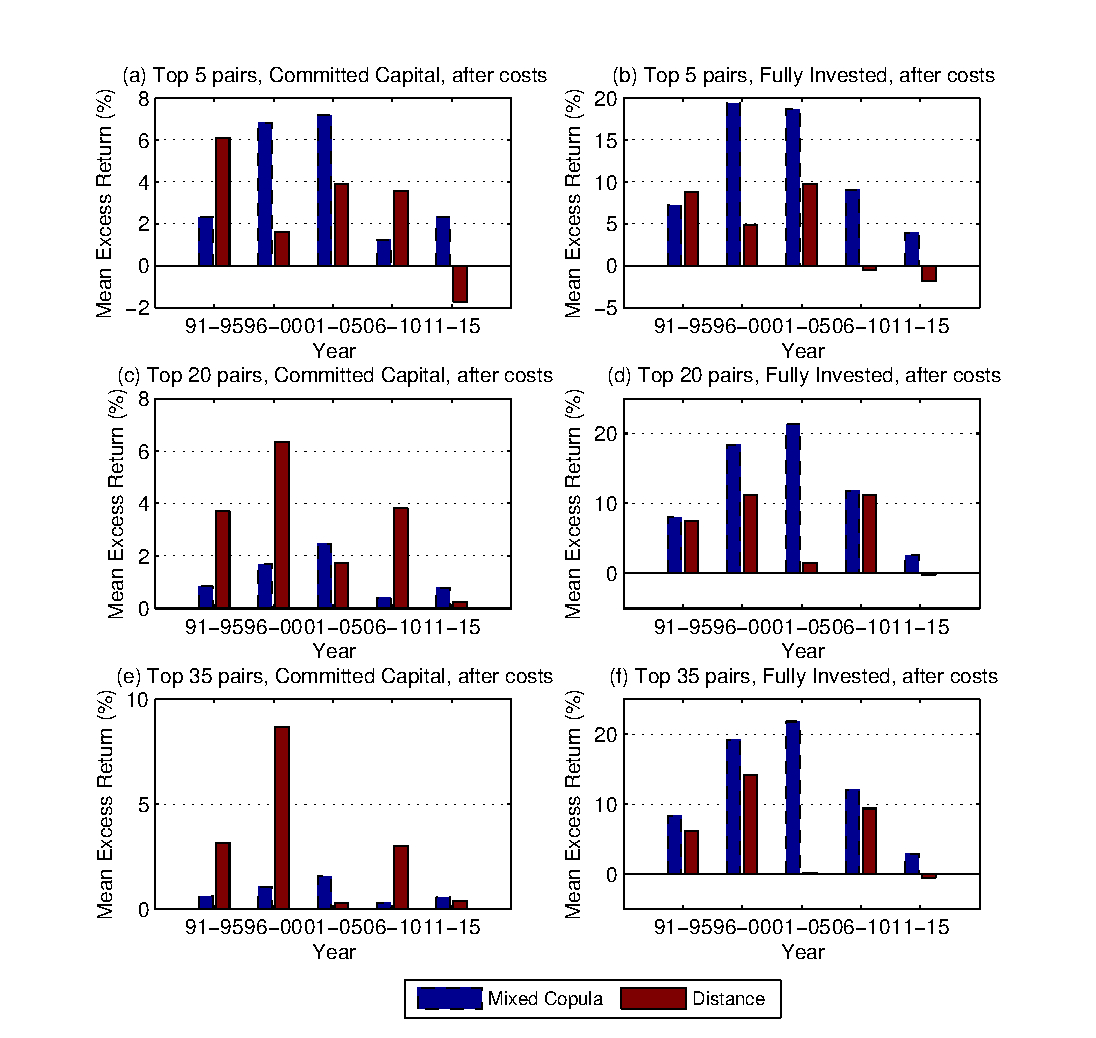
\includegraphics[width=\linewidth]{Figure6.eps}
	\captionsetup{justification=raggedright,
		singlelinecheck=false
	}
	\caption{\textbf{Average excess returns of pairs trading strategies after costs for each sub-period}}
	\caption*{\scriptsize This figure shows how the 5-year rolling window Sharpe ratio densities evolve from July 1996 to December 2015 for each of the strategies.}
	\label{fig:Figure6}
\end{figure}

\begin{figure}[!ht]
	\centering
		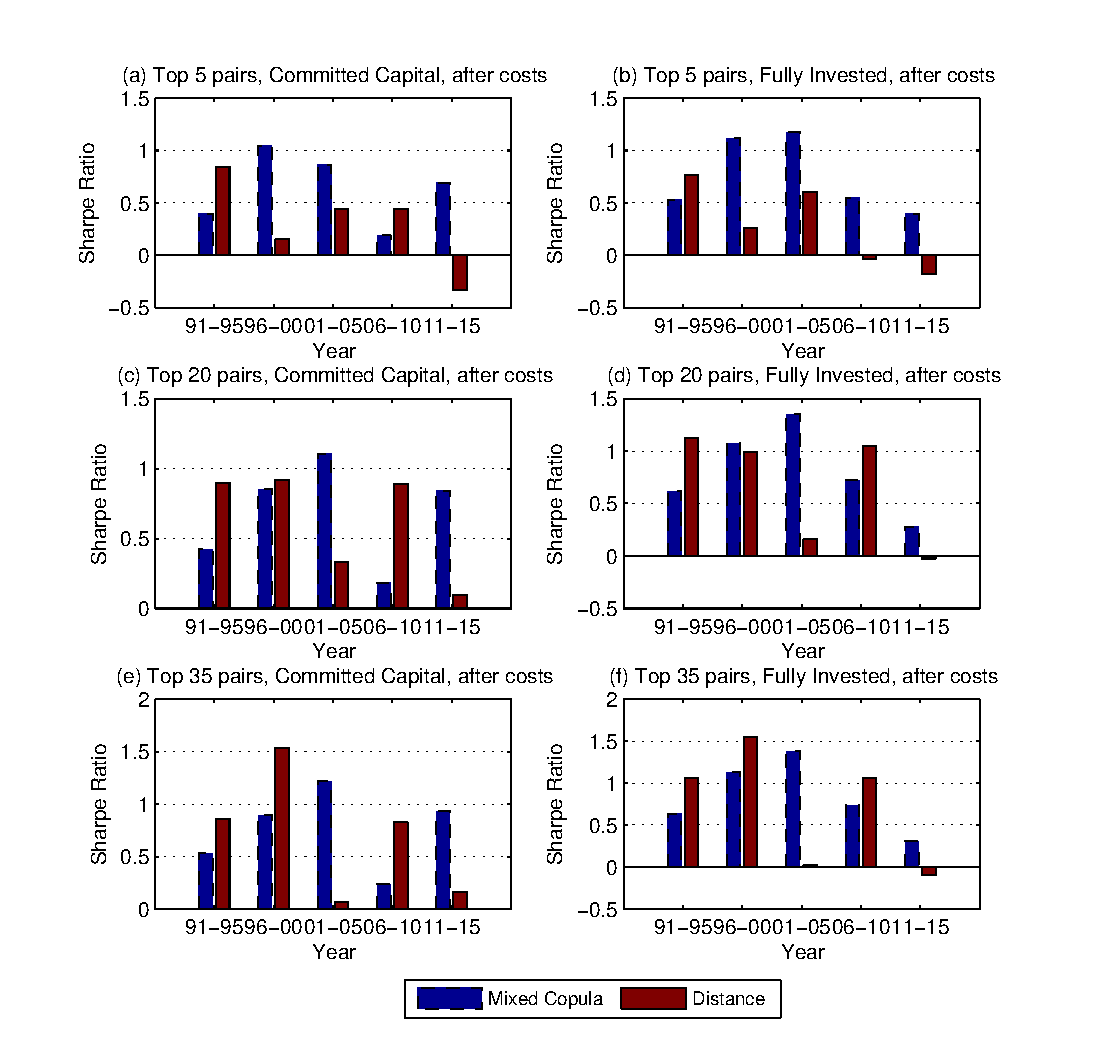
\includegraphics[width=\linewidth]{Figure7.eps}
	\captionsetup{justification=raggedright,
		singlelinecheck=false
	}
	\caption{\textbf{Sharpe Ratio of pairs trading strategies after costs for each sub-period}}
	\caption*{\scriptsize This figure shows how the 5-year rolling window Sharpe ratio densities evolve from July 1996 to December 2015 for each of the strategies.}
	\label{fig:Figure7}
\end{figure}

\vspace{1.0cm}
		\section{Concluding Remarks}
	
Pairs trading fall under the class of statistical arbitrage strategies. It involves a portfolio consisting of long one stock and short the other betting on the empirical fact that the spread among stocks which have strong co-movements tend to return to their historical level.

The main goal of this paper is to verify if a strategy composed of a mixture of copulas is able to generate higher and more robust returns than the distance methodology. We are also interested in understanding better the factors that affect their profitability. 

Using a long-term comprehensive data set spanning 25 years, our empirical analysis suggests that the mixed copula strategy has a superior performance than the distance approach 
when the number of trades is comparable, which occurs for the case of Top 5 pairs.

 
The main findings when the number of trading signals is equiparable are summarized below.
	
	\begin{enumerate}
				
		
	\item The mixed copula strategy is able to generate a higher mean excess return and a Sharpe ratio over twice as much as what we get from investing in the traditional distance method after trading costs. 
	
		
		\vspace{0.3cm}
		
		\item 	The mixed copula approach delivers economically larger alphas than the distance method for both weighting schemes (10 and 58 bps per month on committed and fully invested capital, respectively) after transaction costs, suggesting the importance of the proposed method. It should also be noted that the alphas provided by mixed copula and distance strategies are significant at 1\% and 10\%, respectively, after accounting for several asset pricing factors such as momentum, liquidity, profitability and investment. Thus, the results show that the profits are not fully explained by the other factors.
		
		\vspace{0.3cm}
		
		\item As it can be observed, the right-hand-side tail (of positive outcomes) of the density of the five-year Sharpe ratio is longer for the mixed copula strategy, implying that the copula-based strategy has a better risk-adjusted performance than the distance approach.
		
		\vspace{0.3cm}
		
		\item The share of days with negative excess returns is smaller for the mixed copula approach (41.79\%) than for the distance strategy (46.98\%) and the market performance (47.45\%). 
		
	    \vspace{0.3cm}
		
		
		\item	Neither strategy consistently shows superiority over all subperiods, at least on committed capital. Overall, the mixed copula strategy shows a superior out-of-sample performance relative to the distance approach in the second and third subperiods (1996-2000 and 2001-2005) and after the subprime mortgage crisis (2011-2015), while the distance method delivers a significant better performance in the first (1991-1995) and fourth subperiods (2006-2010) on committed capital. 
		
	\end{enumerate}

\vspace{0.3cm}

We found that the average number of pairs traded per six-month period is only comparable among the strategies for Top 5 pairs in this study. This suggests that a constant two standard deviation threshold \citep{ggr06} is less conservative than the opening trigger point suggested by \citet*{rf15} using the cumulative mispricing indexes $M_{1,t}$ and $M_{2,t}$. Further studies in the application of copulas in pairs trading should investigate the optimal points of entry and exit to make the comparisons more meaningful.


	\newpage
		\section*{Appendix - Regressions on asset pricing factors}
	
	\addcontentsline{toc}{section}{Appendix A - Regressions on asset pricing factors}
	\vspace{0.6cm}
	
	\setcounter{table}{0}
	\renewcommand{\thetable}{A.\arabic{table}}
	
	
	This appendix contains the regressions on asset pricing factors for Top 20 and Top 35 pairs for both strategies.
	
	\vspace{1.0cm}
	

		\begin{table}[!ht]
		\centering \scriptsize
		\caption{Monthly risk profile of Top 20 pairs: \textcolor{blue}{Fama and French} \textcolor{blue}{(2016)}'s five factors plus Momentum and Long-Term Reversal.}
		\begin{threeparttable}[H]
			\begin{tabularx}{\textwidth}{@{\extracolsep{\fill}} lllllllllll@{}}
				\toprule
				\multicolumn{1}{c}{Strategy} & \multicolumn{1}{c}{Intercept} &  \multicolumn{1}{c}{Rm-Rf} &  \multicolumn{1}{c}{SMB} &  \multicolumn{1}{c}{HML} &  \multicolumn{1}{c}{RMW} &  \multicolumn{1}{c}{CMA} & 
				\multicolumn{1}{c}{Mom} &  \multicolumn{1}{c}{LRev} &  \multicolumn{1}{c}{$R^{2}$} & \multicolumn{1}{c}{$R^{2}_{adj}$} \\
				\midrule
				\multicolumn{11}{c}{\textbf{Section 1: Return on Committed Capital}} \\
				\multicolumn{1}{c}{} & \multicolumn{1}{c}{} & \multicolumn{1}{c}{} & \multicolumn{1}{c}{} & \multicolumn{1}{c}{} & \multicolumn{1}{c}{} & \multicolumn{1}{c}{} & \multicolumn{1}{c}{} & \multicolumn{1}{c}{} & \multicolumn{1}{c}{} & \\
				\multicolumn{1}{c}{Distance} & 0.0028 & 0.0056 & -0.0017 & 0.0013 & -0.0031 & 0.0059 & -0.0070 & -0.0068 & 0.028 & 0.027 \\
				\multicolumn{1}{c}{} & $(3.47)^{***}$ & $(5.02)^{***}$ & (-0.63) & (0.38) & (-0.85) & $(1.82)^{*}$ & $(-4.90)^{***}$ & $(-2.37)^{**}$ & & \\
				\multicolumn{1}{c}{Mixed Copula} & 0.0010 & 0.0015 & -0.0006 & 0.0002 & -0.0005 & 0.0007 & -0.0013 & -0.0012 & 0.0091 & 0.008 \\
				\multicolumn{1}{c}{} & $(3.53)^{***}$ & $(3.52)^{***}$ & (-0.75) & (0.22) & (-0.49) & (0.57) & $(-2.19)^{**}$ & (-1.10) & & \\
				
				&       &       &       &       &       &       &       &       &       &       \\
				\midrule
				\multicolumn{11}{c}{\textbf{Section 2: Return on Fully Invested Capital}} \\
				&       &       &       &       &       &       &       &       &       &    \\
				\multicolumn{1}{c}{Distance} & 0.0054 & 0.0103 & -0.0035 & 0.0068 & -0.0050 & 0.0106 & -0.0142 & -0.0121 & 0.030 & 0.029 \\
				\multicolumn{1}{c}{} & $(3.68)^{***}$ & $(5.18)^{***}$ & (-0.55) & (0.90) & (-0.34) & $(1.78)^{*}$ & $(-4.94)^{***}$ & $(-2.08)^{**}$ & & \\
				\multicolumn{1}{c}{Mixed Copula} & 0.0103 & 0.0142 & -0.0088 & 0.0136 & -0.0062 & 0.0086 & -0.0049 & -0.0246 & 0.016 & 0.015 \\
				\multicolumn{1}{c}{} & $(4.50)^{***}$ & $(3.39)^{***}$ & (-1.54) & (1.47) & (-0.70) & (0.75) & (-1.36) & $(-2.36)^{**}$ & & \\
				\bottomrule
			\end{tabularx}
			\begin{tablenotes}
				\item \textit{Note:} \tiny  This table shows results of regressing monthly portfolio return series onto \textcolor{blue}{Fama and French} \textcolor{blue}{(2016)}'s five factors factors plus momentum and long-term reversal over July 1991 and December 2015 (6173 observations). Section 1 shows the Return on Committed Capital and Section 2 on Fully Invested Capital after transaction costs. Pairs are formed based on the smallest sum of squared deviations. The t-statistics (shown in parentheses) are computed using Newey-West standard errors with six lags.
				\item \footnotesize $^{\ast\ast\ast}$, $^{\ast\ast}$, $^{\ast}$  significant at 1\%, 5\% and 10\% levels, respectively.
			\end{tablenotes}
		\end{threeparttable}%
		\label{tab:table104}%
	\end{table}%

\vspace{0.6cm}

		\begin{table}[!ht]
		\centering \scriptsize
		\caption{Monthly risk profile of Top 35 pairs: \textcolor{blue}{Fama and French} \textcolor{blue}{(2016)}'s five factors plus Momentum and Long-Term Reversal.}
		\begin{threeparttable}[H]
			\begin{tabularx}{\textwidth}{@{\extracolsep{\fill}} lllllllllll@{}}
				\toprule
				\multicolumn{1}{c}{Strategy} & \multicolumn{1}{c}{Intercept} &  \multicolumn{1}{c}{Rm-Rf} &  \multicolumn{1}{c}{SMB} &  \multicolumn{1}{c}{HML} &  \multicolumn{1}{c}{RMW} &  \multicolumn{1}{c}{CMA} & 
				\multicolumn{1}{c}{Mom} &  \multicolumn{1}{c}{LRev} &  \multicolumn{1}{c}{$R^{2}$} & \multicolumn{1}{c}{$R^{2}_{adj}$} \\
				\midrule
				\multicolumn{11}{c}{\textbf{Section 1: Return on Committed Capital}} \\
				\multicolumn{1}{c}{} & \multicolumn{1}{c}{} & \multicolumn{1}{c}{} & \multicolumn{1}{c}{} & \multicolumn{1}{c}{} & \multicolumn{1}{c}{} & \multicolumn{1}{c}{} & \multicolumn{1}{c}{} & \multicolumn{1}{c}{} & \multicolumn{1}{c}{} & \\
			\multicolumn{1}{c}{Distance} & 0.0026 & 0.0060 & -0.0009 & -0.0010 & 0.0014 & 0.0060 & -0.0066& -0.0053 & 0.034 & 0.033 \\
			\multicolumn{1}{c}{} & $(3.93)^{***}$ & $(5.55)^{***}$ & (-0.54) & (-0.50) & (0.41) & $(1.96)^{**}$ & $(-5.38)^{***}$ & $(-1.99)^{**}$ & & \vspace{.1cm}\\
			\multicolumn{1}{c}{Mixed Copula} & 0.0007 & 0.0009 & -0.0003 & -0.0000 & -0.0004 & 0.0007 & -0.0007 & -0.0007 & 0.009 & 0.008 \\
			\multicolumn{1}{c}{} & $(3.96)^{***}$ & $(3.81)^{***}$ & (-0.69) & (-0.04) & (-0.69) & (0.98) & $(-2.17)^{**}$ & (-1.14) & & \\
				&       &       &       &       &       &       &       &       &       &       \\
				\midrule
				\multicolumn{11}{c}{\textbf{Section 2: Return on Fully Invested Capital}} \\
				&       &       &       &       &       &       &       &       &       &    \\
		
		\multicolumn{1}{c}{Distance} & 0.0049 & 0.0111 & -0.0033 & -0.0000 & 0.0014 & 0.0140 & -0.0127 & -0.0114 & 0.037 & 0.036 \\
		\multicolumn{1}{c}{} & $(4.07)^{***}$ & $(5.36)^{***}$ & (-0.90) & (-0.31) & (0.49) & $(2.56)^{**}$ & $(-5.47)^{***}$ & $(-2.04)^{**}$ & & \vspace{.1cm}\\
		\multicolumn{1}{c}{Mixed Copula} & 0.0106 & 0.0146 & -0.0085 & 0.0130 & -0.0070 & 0.0100 & -0.0049 & -0.0251 & 0.017 & 0.016 \\
		\multicolumn{1}{c}{} & $(4.63)^{***}$ & $(3.48)^{***}$ & (-1.50) & (1.40) & (-0.79) & (0.87) & (-1.36) & $(-2.41)^{**}$ & & \\
				\bottomrule
			\end{tabularx}
			\begin{tablenotes}
				\item \textit{Note:} \tiny  This table shows results of regressing monthly portfolio return series onto \textcolor{blue}{Fama and French} \textcolor{blue}{(2016)}'s five factors factors plus momentum and long-term reversal over July 1991 and December 2015 (6173 observations). Section 1 shows the Return on Committed Capital and Section 2 on Fully Invested Capital after transaction costs. Pairs are formed based on the smallest sum of squared deviations. The t-statistics (shown in parentheses) are computed using Newey-West standard errors with six lags.
				\item \footnotesize $^{\ast\ast\ast}$, $^{\ast\ast}$, $^{\ast}$  significant at 1\%, 5\% and 10\% levels, respectively.
			\end{tablenotes}
		\end{threeparttable}%
		\label{tab:table105}%
	\end{table}%

\newpage
	
		
	\addcontentsline{toc}{section}{References}
	\bibliographystyle{rfs}
	\bibliography{mypapers}
	

	\end{document} 